\documentclass[notitlepage]{report}
\usepackage[utf8]{inputenc} % Prendre en compte les caractères accentués
%\usepackage[francais]{babel} % Prendre en compte les particularités de la typographie française.
\usepackage{geometry}         % marges
\usepackage{graphicx}         % images
\usepackage{setspace}
%\usepackage[french]{varioref}
\usepackage{titlesec}
\usepackage{parskip}
\usepackage{url}
\usepackage{verbatim}
\usepackage{caption}
\usepackage{enumitem}
\usepackage{ragged2e}
\usepackage{xcolor}
\usepackage{textcomp}
\usepackage{listings}
\usepackage{pgfgantt}
\usepackage{lscape}
\usepackage{pdfpages}
\usepackage{supertabular} % tableaux qui tiennent sur plusieurs pages
\usepackage{multirow} % plusieur ligne dans une ligne de tableau
\usepackage{pdflscape} % Automatic rotation of the landscape page
\usepackage{colortbl} %Couleur de fond tableau
\usepackage{lipsum,etoolbox} %Pour que l'abstract se mette dans la ToC
\usepackage{subcaption} %image side by side
\usepackage{amsmath} % Maths matrix 
\usepackage{amssymb} % Maths matrix

\newgantttimeslotformat{stardate}{%
	\def\decomposestardate##1.##2\relax{%
		\def\stardateyear{##1}\def\stardateday{##2}%
	}%
	\decomposestardate#1\relax%
	\pgfcalendardatetojulian{\stardateyear-01-01}{#2}%
	\advance#2 by-1\relax%
	\advance#2 by\stardateday\relax%
}

\titlespacing{\chapter}{0pt}{*-5}{*5}
\titlespacing{\section}{0pt}{*2}{*2}
\titleformat{\chapter}[hang]{\bf\huge}{\thechapter}{2pc}{}
%\titleformat{\chapter}[hang]{\bf\huge}{\thechapter}{14pt}{\LARGE}
\renewcommand{\baselinestretch}{1.2}
\setlength{\parskip}{1.5ex plus .4ex minus .4ex}
\setlength{\parindent}{15pt} 
\setlength{\topmargin}{-35pt}
\setlength{\textheight}{600pt}

\makeatletter
% subsubsubsection
\newcounter{subsubsubsection}[subsubsection] 
\renewcommand\thesubsubsubsection{\@roman\c@subsubsubsection}
\newcommand\subsubsubsection{\@startsection{subsubsubsection}{4}{\z@}%
                                     {-3.25ex\@plus -1ex \@minus -.2ex}%
                                     {1.5ex \@plus .2ex}%
                                     {\normalfont\small\bfseries}}
\newcommand*\l@subsubsubsection{\@dottedtocline{3}{5.2em}{1em}}
\newcommand*{\subsubsubsectionmark}[1]{}
\setcounter{secnumdepth}{2}
\makeatother

 
\begin{document}
\sloppy % Justification moins stricte : des mots ne dépasseront pas des paragraphes

\newcommand{\reporttitle}{Immersive Virtual Reality System}     % Titre
\newcommand{\reportsubtitle}{SIGVerse interaction trough Robot Operating System}     % SousTitre
\newcommand{\reportauthor}{Geneviève \textsc{Cirera} (SI5 - Web)} % Auteur
\newcommand{\reportsubject}{Final report} % Sujet
\newcommand{\HRule}{\rule{\linewidth}{0.5mm}}
\setlength{\parskip}{1ex} % Espace entre les paragraphes

\begin{titlepage}

\begin{center}

\begin{minipage}[t]{0.49\textwidth}
\vspace*{-2cm}
  \begin{flushleft}
    
\includegraphics [width=55mm]{images/LogoUNSA.jpg} \\[0.6cm]
    
  \end{flushleft}
\end{minipage} 
\begin{minipage}[t]{0.49\textwidth}
  \begin{flushright}
    
\includegraphics [width=55mm]{images/Logo_polytech_SI.jpg} \\[0.2cm]
  \end{flushright}
\end{minipage} \\[2.0cm]
\vspace*{-1cm}
\textsc{\Large Computer Science Engineer}\\[0.5cm]
\textsc{\Large \reportsubject}\\[0.5cm]
\HRule \\[0.4cm]
{\huge \bfseries \reporttitle}\\[0.4cm]
{\Large \bfseries \reportsubtitle}\\[0.2cm]
\HRule \\[1.5cm]
\vspace*{-1cm}
\begin{minipage}[t]{0.64\textwidth}
  \begin{flushleft} \large
    \emph{Intern :}\\
    \reportauthor
  \end{flushleft}
\end{minipage}
\begin{minipage}[t]{0.35\textwidth}
  \begin{flushleft} \large
    \emph{Tutor :} \\
    Frédéric \textsc{Precioso} \\[0.5cm]
    \emph{Supervisor :} \\
    Inamura \textsc{Tetsunari}
  \end{flushleft}
  \vspace*{0.8cm}
\end{minipage}
%\vspace*{7.0cm}
\textsc{\Large Enterprise\\National Institute of Informatics\\(Tokyo - Japan)}\\[0.5cm]
{\emph{2015 March, 15 - 2015 August, 30}}\\
\vspace*{0.8cm}
%\textsc{\Large Abstract}\\[0.5cm]
%\justify
%Résumé
\vfill

%{\large 5 mars 2012}
\center
\vspace*{0.2cm}

\includegraphics [width=80mm]{images/nii_logo.png} \\[0.6cm]
\end{center}

\end{titlepage}

%\chapter*{Remerciements}
%\setlength{\parskip}{2.5ex plus .4ex minus .4ex}
\setcounter{page}{2} 
%Je tiens à remercier certaines personnes sans lesquelles ce stage n'aurait pas eu lieu.\\
%Hélène Raynal, responsable du projet RECORD\footnote{Rénovation et CooRDination de la modélisation de cultures pour la gestion des agro écosystèmes}, Gauthier Quesnel du projet VLE\footnote{Virtual Laboratory Environment}, appartenants au département MIA\footnote{Mathématiques et Informatique Appliquées}.\\
%Laurence Puillet et Olivier Martin, du projet Archimod, département PHASE\footnote{PHysiologie Animale et Systèmes d’Élevage} qui ont exprimé les besoins et sont les principaux futurs utilisateurs ainsi que Régis Sabbadin, Directeur de l'Unité MIAT\footnote{Mathématiques et Informatique Appliquées de Toulouse}, lieu de déroulement du stage.\\
%
%Merci également à mon maître de stage Patrick Chabrier pour ses explications et conseils tout au long du stage ainsi que les stagiaires présents dans l'entreprise qui m'ont aidé et rendu le temps passé dans l'entreprise très agréable.\\
%
%Je souhaite également remercier toutes les personnes au sein de l'école Polytech'Nice qui ont rendu ce stage possible.
\renewcommand{\abstractname}{Gratitude}
\vspace*{\fill}
\begin{abstract}
%\addcontentsline{toc}{chapter}{Gratitude}
I wish to thank the National Institute of Informatics who gave me the opportunity to do my six-month internship in one of its laboratory. With this internship, I finalize my master's degree in computer science engineering.\\

I also want to thank my supervisor, Inamura \textsc{Tetsunari} associate professor, for his time invested, his interest in my study and for all the knowledge he helped me deepen.\\

I thank the National Institute of Informatics administration staff who helped me get over all administrative steps and my interrogations. Also a thank you to Polytech'Nice Sophia who make this internship possible.\\

Finally I would like to say many thanks to all the people who made my study and internship possible, and encourage me during my all study - friends, familly and the all people I met who gave me good moment.
\end{abstract}
\vspace*{\fill}
\renewcommand{\abstractname}{Abstract}

%\setcounter{page}{2} 
\tableofcontents % Table des matières

\chapter{Introduction}
\setlength{\parskip}{2.5ex plus .4ex minus .4ex}
\section{Context}
\subsection{National Institute of Informatics}
The NII\footnote{National Institute of Informatics} of Tokyo is an inter university research institute which aim to develop the research in multiple domains. The Institute is focused on informations-related fields including networking software and content.
The NII is composed by several laboratories which work on different international research project. One of them is directed by the associate professor Inamura Tetsunari where I am doing my internship.\\
The Inamura laboratory works on several project, which one is SIGVerse, a simulator.

\subsection{SIGVerse}
SIGVerse is a virtual world which can modelise objects and agents.\\
This simulator has been created to give a tool for studying interactions between agents but also comprehension and knowledge in many fields.\\
Understanding the mecanism of intelligence of human being is the key to develop intelligent robot system. That's why this simulator is very useful.\\
The movement of the user can be reproduced in the virtual world thanks to the kinect and the representation of the world can be projected on the oculus. So, the user can be ``inside'' the simulator and interact more easily with its.\\
We can see in figure~\ref{fig:manVirtualWorld}, the representation of an agent. This agent could be a robot too, and it is possible to program its movements or send to it a message to execute an action. That's why this simulator is well adapted to host the training and virtual competition of Robocup.\\
However, the use of the simulator is exclusively for SIGVerse users which limits its growth.\\

\noindent\begin{minipage}{\linewidth}% to keep image and caption on one page
\makebox[\linewidth]{%        to center the image
  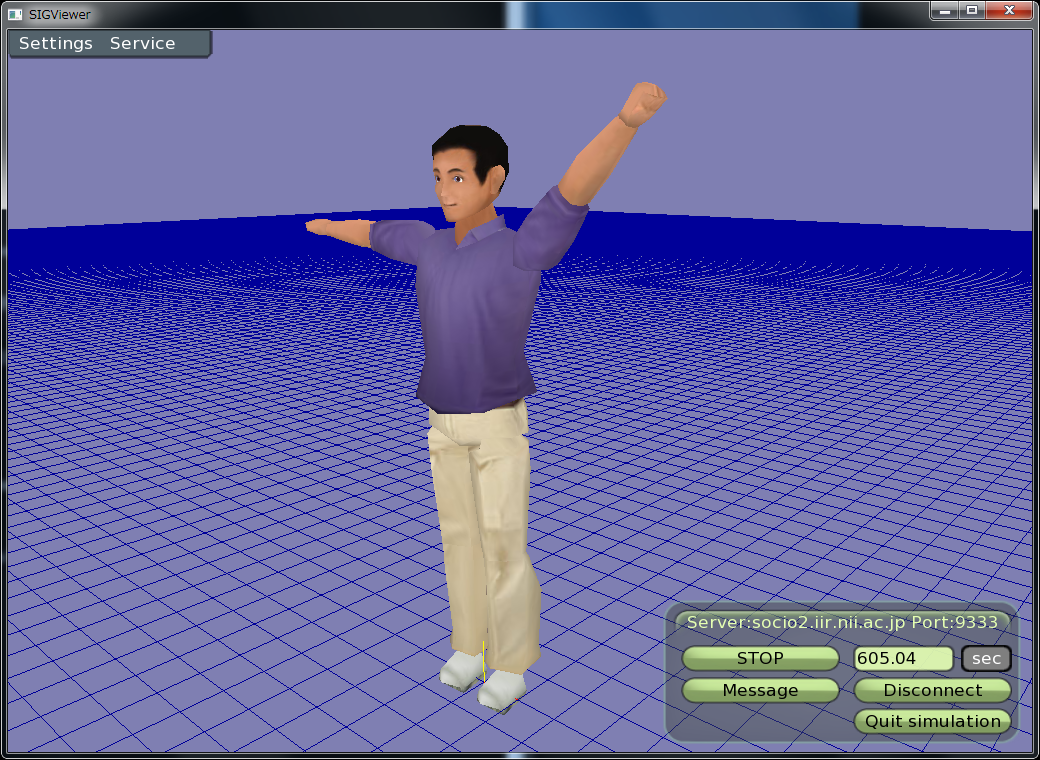
\includegraphics [width=100mm]{images/manViewer.png}}
\captionof{figure}{Simple agent in the virtual world}\label{fig:manVirtualWorld}%      only if needed  
\end{minipage}

\section{Topic}
SIGVerse is limited to SIGVerse users. This topic has the goal to growth the SIGVerse community by joining the ROS\footnote{Robot Operating System} community.\\
This gathering has been chosen because of several reasons.\\
First of all ROS is open source like SIGVerse and has a big community who works on robots. Then ROS can provide a collection of tools, libraries, and conventions that aim to simplify the task of creating complex and robust robot behavior across a wide variety of robotic platforms.\\
ROS make possible to manage a robot as SIGVerse do but there is advantages to using ROS. Indeed, ROS is designed to be as distributed and modular as possible so, it encourages the collaboration to develop robot software whereas SIGVerse is not.\\

In this report, I am going to detail the suggested work, general idea and how ROS works. After that, I am going to detail what I started doing, architecture, topics, services, troubles...

\include{context}

\chapter{Suggested work}
\setlength{\parskip}{2.5ex plus .4ex minus .4ex}
\section{Robot Operating System}\label{sec:ROS}
The ROS\footnote{Robot Operating System} is an open source flexible framework for writing robot software. It is a collection of tools, libraries, and conventions that aim to simplify the task of creating complex and robust robot behavior across a wide variety of robotic platforms.\\
%ROS make possible to manage a robot as SIGVerse do but there is advantages to using ROS. Indeed, ROS is designed to be as distributed and modular as possible so, it encourages the collaboration to develop robot software whereas SIGVerse is not.\\
%ROS provides more than 3,000 packages and integration points for services like hardware drivers, useful external librairies,... So, everything possible with SIGVerse would be though ROS.\\
%Moreover, ROS use URDF\footnote{Unified Robot Description Format} for describing agents, which consists of an XML document like the agent description on SIGVerse.\\
At the lowest level, ROS is commonly referred to as a middleware. It provides some facilities like publishing/subscribing anonymous message passing and request/response remote procedure calls. We can see in the figure~\ref{fig:concept_de_base_ROS} the base concept of ROS. Each entity is a node who can publish or subscribe to a topic. If a node publish to a topic, every node who subscribed to it will receive the message. Many nodes can publish in the same topic and many nodes can subscribe to the same topic. Every node can publish and/or subscribe to several nodes.\\
We can also see a service between two nodes, the first node can send a request with zero or more parameters to the other node who will act and respond with parameters.

\noindent\begin{minipage}{\linewidth}% to keep image and caption on one page
\makebox[\linewidth]{%        to center the image
  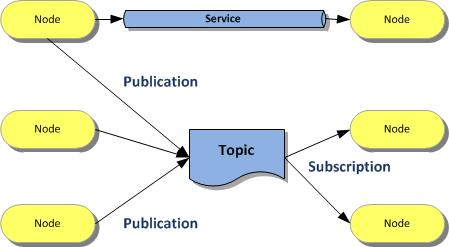
\includegraphics [width=140mm]{images/Concepts-de-base-ROS.jpg}}
\captionof{figure}{Publish/Subscribe system}\label{fig:concept_de_base_ROS}%      only if needed  
\end{minipage}

%Moreover, respect to the ROS alternatives like Mobile Robot Programming Toolkit, Microsoft Robotics Developer Studio or CARMEN, ROS has been choose for is big community, that will increase the number of users.\\

\section{SIGVerse architecture}
Currently, the architecture of SIGVerse is as shown figure~\ref{fig:SIGVerseSimple}.\\
On the Linux part, the server is running with the xml file where the agent is defined and the Controller.cpp where the initialisation and actions are defined.\\
On the Windows part, two things, SIGViewer which is a GUI and aim to show to the user the agent on the simulator. The services are all devices which can provide data to the server. That means the kinect, the oculus,...\\

\noindent\begin{minipage}{\linewidth}% to keep image and caption on one page
\makebox[\linewidth]{%        to center the image
  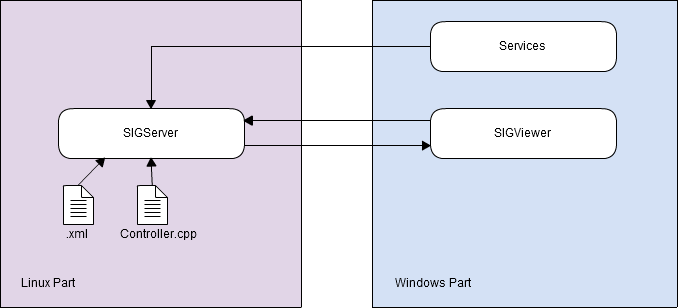
\includegraphics [width=120mm]{images/SIGVerseSimple.png}}
\captionof{figure}{SIGVerse}\label{fig:SIGVerseSimple}%      only if needed  
\end{minipage}

\section{Objective}
As seen section~\ref{sec:ROS}, using ROS to create and manipulate agents on SIGVerse will be very useful. So, I have to design and develop an interface between SIGVerse and ROS.\\
This interface has to make available the features of SIGVerse from ROS, that means initializing one or more agents, make them act and make the services working though ROS.\\
The agents can be: robot, human or object.\\
The expected architecture is shown figure~\ref{fig:SIGVerseROS}. We can see the SIGServer and the ``Controller'' inside the ROS interface, that means the user will not need to interact with SIGVerse, he only defined the agent in the xml file and then, interacting with ROS, send messages to the server though the interface. The user will not need to write the ``Controller'', it will be automatically generated.\\
This is an example with one xml file and one controller, but it will be necessary to generalise it to more than one.

\noindent\begin{minipage}{\linewidth}% to keep image and caption on one page
\makebox[\linewidth]{%        to center the image
  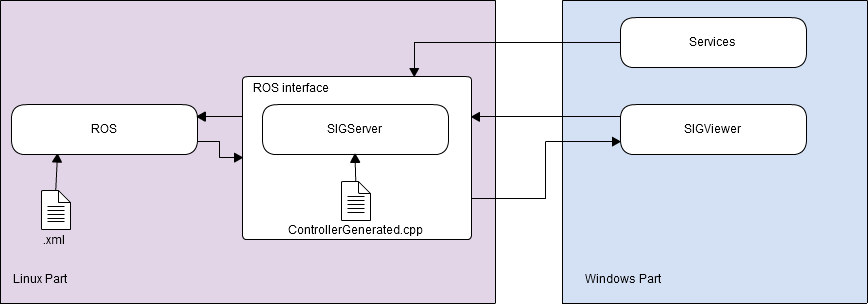
\includegraphics [width=150mm]{images/SIGVerseROS.png}}
\captionof{figure}{SIGVerse with ROS interface}\label{fig:SIGVerseROS}%      only if needed  
\end{minipage}

\section{Functionalities requiered}
\subsection{General requirement} %Besoins généraux
Currently, SIGVerse has two parts: SIGServer and SIGViewer and they communicate directly together as seen figure~\ref{fig:SIGVerseSimple}.\\
The aim is to find a way for the ROS users for using SIGVerse. That means the ROS user will only write ROS code and this will be enough for manipulate the simulator.\\
Right now, if the ROS user wants to do it, he has to make the interface himself, mapping the SIGVerse function which is needed. That is why, a common interface with the main functions are useful. After that, the user will have the possibility to enhance it.\\

Three agents are available on SIGVerse: the robot, the human and the object and different actions are available for each one. But some same actions are available for many of them. Indeed the robot agent inherits from the object agent and the human can be a special robot.

\subsection{Use case}
The main use case is for the Robocup competition. Indeed, with this interface, ROS users could participate to the competition.\\
RoboCup is an annual international robotics competition founded in 1997.\\
There are many stages of competition, RoboCupRescue, RoboCup@Home, RoboCupJunior,...\\
The best known is the football competition where two team of robots are playing football, but the Inamura lab works on RoboCup@Home using SIGVerse. Three kinds of task are competing, the clean up task, the follow me and the EGPSR task.\\
In a simple clean up task, the robot detects the trash, go to take it and puts it in the trashbox detected. Points are given for every good things done like ``take the trash'' and ``put it in the trashbox'', but points are removed if a collision occurs.\\
The aim of the follow me task is to follow someone without collision, don't lose him and knowing in which direction after entering the elevator. Indeed, if the man entry the elevator, the robot will enter too but the man will not be able to go out before the robot do it.\\
The EGPSR task is the interaction between the human and the robot. The man asks the robot for an object in a room and the robot has to go to the right room and get it back.\\
First of all, the clean up task has to work with ROS, that means the methods used with the robot and some methods of objects.\\
After that, there is a third agent, the human, so the follow up task will be a pertinent example.

\subsection{To go further}
To go further, the adaptation of some ROS functionalities to SIGVerse will be a great advantage for SIGVerse. Indeed, some actions can take a lot of time to program inside SIGVerse whereas just few information can be needed by a ROS package to obtain the same information.\\
Two packages ROS are suggested, SLAM\footnote{Simultaneous Localization And Mapping} and ik\footnote{Inverse Kinematics}.

\subsubsection{SLAM}
The SLAM problem appears like the chicken and egg problem. Indeed, it is the fact of creating the map at the same time as localizing himself inside the map.

The main reason of this package choose is because inside SIGVerse, the robot know the map because it is inside a simulator and has access to it. I think to be closer the reality, the robot has to discover the map and no taking it and making his path planning.

As explained on the ros tutorial of the slam\_gmapping package, this package can be used like a black box. We only need to know what the package need as entry and what it will produce.

\subsubsection{Inverse Kinematics}
Inverse kinematics is the use of the kinematics equations in order to provide the desired position of the end effector. That means, with the defined position of the end effector, the inverse kinematics found the position of all joints of the arm.\\

This choice is due to the observation of this lack of this functionnality very important inside SIGVerse. Indeed, to program the user side of the Robocup demonstration, grasping an object with an arm was not instinctive at all. The user has to find each angle (shoulder, elbow,...) by himself and animate  the arm. %(trigger the movement of the arm)
 

\section{ROS and SIGVerse}
On SIGVerse an agent is defined by an XML file for his representation and a ``controller'' for his dynamic. The dynamic allows an agent to act, receive message or send message.\\
Currently, the user has to transform the ``Controller'' into a ROS node himself, defining the interface for each method needed.\\
We can see in figure~\ref{fig:sig_ros} an example. Indeed, we can see the ``Controller'' inside the server who is also a ROS node. That is why it can publish a message to a topic and subscribe to ``Velocity Topic''. After that, any ROS node can be created and publish or subscribe to topics, the SIGVerse agent can receive instructions from a topic or a service.\\

In this example figure~\ref{fig:sig_ros} given on the SIGVerse wiki page\cite{SIGVerseWikiROS}, the ``Controller'' launch the ROS node when the simulation starts and the topics are created. However, we want the user to write only ROS code and do not bother himself with the ``Controller'' and SIGVerse functioning.
\noindent\begin{minipage}{\linewidth}% to keep image and caption on one page
\makebox[\linewidth]{%        to center the image
  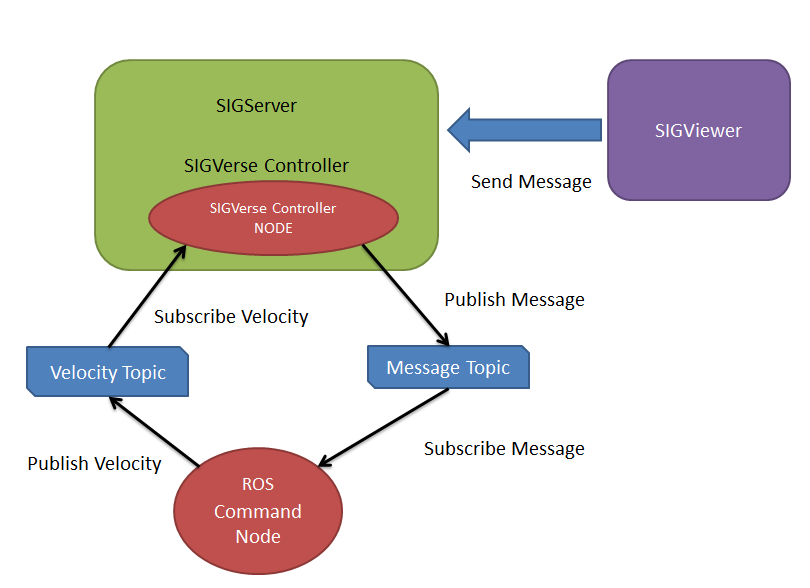
\includegraphics [width=150mm]{images/sig_ros.png}}
\captionof{figure}{SIGVerse controller sending and receiving message}\label{fig:sig_ros}%      only if needed  
\end{minipage}

%L'objectif est de pouvoir modéliser en spécifiant au sein d'un système dynamique des populations d'individus.\\
%Un individu est formalisé par un système d'équations différentielles et tous les individus d'une population se réfèrent au même système d'équations différentielles.\\
%Au sein d'une population les individus peuvent différer de par la valeur de leurs paramètres mais ce n'est pas une obligation.\\
%\\
%La dynamique des populations est définie par un ensemble d’événements portant sur les individus. Un évènement est défini par des conditions d'activation et des effets.\\
%Les conditions d'activation sont exprimées en fonction du temps de la simulation ou de l'état du système simulé. L'état du système est l'union de tous les états des individus.\\
%Il existe 3 types d'effet: Création d'un individu, suppression d'un individu et réinitialisation d'un individu.

%\subsection{Structure du modèle DEVS}
%Chaque individu est un système d'équations différentielles défini par une classe C++. Cette classe est appelée classe d'individu. C'est elle qui doit être défini par l'utilisateur puis qui servira de base pour créer tous les individus de ce type là. C'est pourquoi chaque individu de même type, a la même dynamique, seuls les paramètres peuvent varier entre eux si l'utilisateur souhaite en modifier un ou plusieurs.\\
%Chaque individu est indépendant, ils n'intéragissent pas directement les un avec les autres. Ils doivent communiquer par l'intermédiaire d'un même controleur auquels ils sont tous connectés.\\
%Chaque port de sortie de chaque individu est relié aux ports d'entrée du controleur, ce qui permet à ce dernier de recevoir des évènements, les traiter et envoyer des réponses adéquates par l'intermédiaire de ses ports de sortie reliés à chaque individu par des ports d'entrée.\\
%Lors de la simulation, la dynamique du controleur se met en marche. Elle initialise tous les individus, exécute sa dynamique interne, reçoit les évènements externes et envoie des réponses aux individus. Durant la simulation, le controleur peut à tout moment, créer un nouvel individu, en supprimer ou en modifier les paramètres grâces aux évènements qu'il reçoit en entrée et qu'il peut envoyer en sortie.\\
%Par exemple :\\
%\noindent\begin{minipage}{\linewidth}% to keep image and caption on one page
%\makebox[\linewidth]{%        to center the image
%  \includegraphics [width=150mm]{images/exemple_ibm.png}}
%\captionof{figure}{Trois Loups créés par le controleur lors de la simulation}%\label{visina8}%      only if needed  
%\end{minipage}

%Le controleur crée les individus ``Loup 1'', ``Loup 2'' et ``Loup 3'' qui sont bien indépendants les uns des autres et tous reliés au controleur comme expliqué au paragraphe précédent. \\
%
%\subsection{IBM dans VLE}
%Dans VLE, chaque système ou simulation est représenté par un Vpz qui est un fichier xml où est décrit tout le système. Modèles présents (individus), conditions expérimentales (valeurs des paramètres), classes d'individus, ports d'entrées et de sorties...\\
%Dans le Vpz, un controleur est obligatoirement présent s'il s'agit d'un système IBM. Il se crée automatiquement lors de la première ouverture du plugin IBM. \\Ensuite, les modèles souhaités par l'utilisateur sont créés lors de la simulation par le controleur grâce aux classes d'individu définies dans le vpz.\\
%Par exemple : \\
%\noindent\begin{minipage}{\linewidth}% to keep image and caption on one page
%\makebox[\linewidth]{%        to center the image
%  \includegraphics [width=160mm]{images/vpz1.png}}
%\captionof{figure}{Composition d'un Vpz}%\label{visina8}%      only if needed  
%\end{minipage}
%
%Ici, le controleur crée n Loups et m Moutons lors de la simulation, mais seul le modèle ``Controleur'' est présent dans le vpz. Le controleur est cependant lié aux classes ``Loup'' et ``Mouton'' afin de pouvoir créer les individus.

%\section{Fonctionnalités du plugin}
%À son ouverture, le plugin récupère toutes les classes d'individu déjà présentes dans le Vpz. Il offre ensuite la possibilité d'ouvrir le plugin Forrester afin de créer d'autres classes et modifier ou supprimer les classes existantes.\\
%Afin de manipuler les individus lors de la simulation, le plugin propose un champs de texte afin que l'utilisateur exprime ces besoins par l'intermédiare d'un petit langage simple appelé Lua et quelques extensions que j'aurai développées.\\
%Ces besoins peuvent être multiple, ils peuvent avoir un effet sur les individus, création, suppression, modification ou bien renvoyer des informations, valeur d'une variable, nombre d'individus, identifiant d'un individu...\\
%D'autre part, le plugin crée automatiquement un exécutive appelé ``Controleur'' à son ouverture. Controleur qui sera chargé de manipuler les individus selon le script qu'aura écrit l'utilisateur, et la dynamique DEVS.\\

\chapter{Work performed}
\setlength{\parskip}{2.5ex plus .4ex minus .4ex}
\section{Controller}\label{sec:controller}
Each ``Controller'' associated to an agent on the world inherit from the main class ``Controller'' of SIGVerse. That is why each of them has the same dynamic shown figure~\ref{fig:controllerDyn}.\\

When the simulation starts on the SIGViewer, each ``Controller'' is initialized running ``onInit'' method. After that the ``onAction'' method is running regularly, it can be every 1 seconds like 0.1, 0.5,... It is defined by the return value of ``onAction'' method.\\
If a collision occurs between the agent and something else, ``onCollision'' is executed.\\
If the agent receives a message, ``onRecvMsg'' is executed.\\

In any case, ``onAction'' is running until the simulation stops. If the simulation restarts, ``onInit'' is not executed, the simulation continues where it stopped.\\

\noindent\begin{minipage}{\linewidth}% to keep image and caption on one page
\makebox[\linewidth]{%        to center the image
  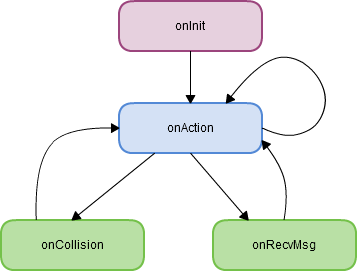
\includegraphics [width=100mm]{images/controllerDyn.png}}
\captionof{figure}{Dynamic of the ``Controller''}\label{fig:controllerDyn}%      only if needed  
\end{minipage}

\section{Architecture}
\subsection{General objective}
On the SIGServer, severals ``Controller'' can run at the same time, because there are one for each agent in the simulator and their types can be different. For exemple, we can have a ``Controller'' for a Robot and ``Controller'' for an object. The principal difference between them is that a Robot controller do not apply the same method to the agent than an object, indeed the robot can move, not an object. But they have the same dynamic, section~\ref{sec:controller}.\\
If we have three robots in the simulator, that means three ``Controller''.\\

We can see figure~\ref{fig:sig_ros_general} how the interface has to work. Several nodes can send information to topics which can be the same or not. This is the ROS part. And these topics are subscribed by the ``Controller'' of SIGServer.\\
As we can see, the same node can publish to the same node ``Topic 4'' or one node can publish to several nodes ``Node 1''.\\
However, different ``Controller'' cannot publish or subscribe to the same topic. The reason is that the ROS user do not have to write the ``Controller'' or edit it neither, it will be generated and I can not know if the user want the same behaviour between two or more agents. If the user wants this behaviour, he will have to send the same message to severals topics.\\

As we can see figure~\ref{fig:sig_ros_general} a service can be called too. The difference with publishing/subscribing is that a request is sent and the ``Controller'' will answer with a response to the node who asked ``Node 3''.

\noindent\begin{minipage}{\linewidth}% to keep image and caption on one page
\makebox[\linewidth]{%        to center the image
  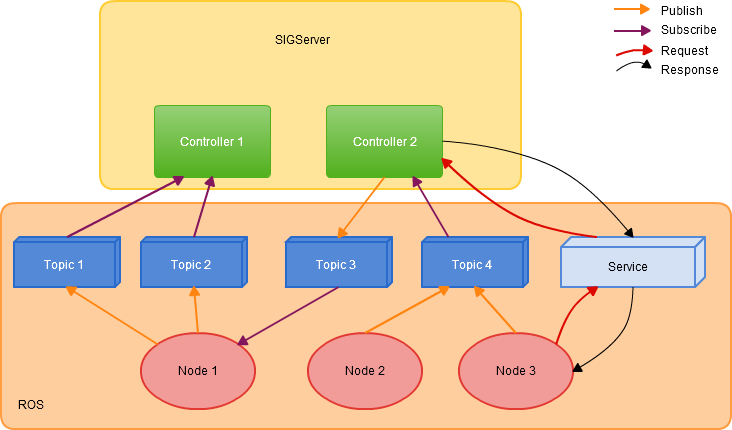
\includegraphics [width=150mm]{images/sig_ros_general.png}}
\captionof{figure}{Many ROS nodes send and receive information to many controllers}\label{fig:sig_ros_general}%      only if needed  
\end{minipage}

\subsection{Controllers used}
As explained earlier, one ``Controller'' is associated to one agent for making him act. This association is defined in the xml file which describes the agent.\\
The same ``Controller'' can be associated to several agents, that means that all agent associated to this ``Controller'' will act the same.\\
On this project, ``Controllers'' has to be developped for creating topics which sent information and make the agent acting. So, two ``Controllers'' will be necessary, one for the robot and one for the object. For generals methods like getting entities, they can be included on the object controller.\\
The best would be a general controller for the methods in common to avoid the duplication of topics, but for this mid-term report, only the robot controller and the object controller are implemented with the methods inside them.\\
So, in our case, I have as many topics (or services) for getting entities as number of agent in the simulator.\\

The robot ``Controller'' inherits from the object ``Controller'' called ``SimObjController''. The reason is that in SIGVerse, a robot is an object and has only two methods more than on the object ``Controller''.\\

\subsection{Package}
ROS is an open source framework who works with packages, every extension is a package. So, the ROS users just need to download the package wanted.\\
That is why I choose to develop a package, and only running the node called ``ros\_controller'' will be necessary to launch the SIGServer, create the ``Controllers'', the topics and services.\\
We can see figure~\ref{fig:sig_ros_package} the composition of the package.
\begin{description}
	\item[src] : The generic ``Controller'' for each kind of agent more the principal node ``ros\_controller'' for launchin the package.
	\item[srv] : The definition of each services needed.
	\item[msg] : The definition of each messages needed.
	\item[tests] : Tests files to check the validity of the implementation.
	\item[doc] : Documentation useful for the use of the package, this report and a user manual.
	\item[robot\_desc] : Contains files for the description of Hiro robot and the scripts necessary to his modification in order to use the ik package.
\end{description}

\noindent\begin{minipage}{\linewidth}% to keep image and caption on one page
\makebox[\linewidth]{%        to center the image
  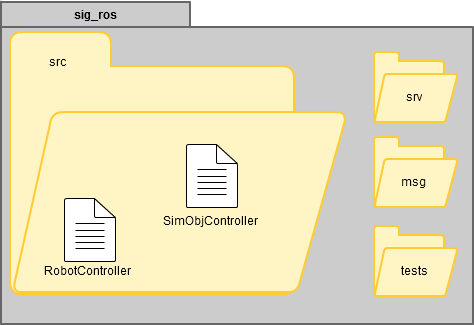
\includegraphics [width=120mm]{images/package_sig_ros.png}}
\captionof{figure}{sig\_ros package}\label{fig:sig_ros_package}%      only if needed  
\end{minipage}

\section{Usage}
From the user's point of view, three steps are important, see figure~\ref{fig:usage}.\\
First, the user launches the sig\_ros package. So, the SIGServer is automatically launched and the SIGViewer can be connected.\\
Second, the user starts the simulation from the SIGViewer. So, all topics and services are created and linked to the ``Controller'' thanks to the package sig\_ros.\\
Finally, the user can create all the ROS node he wants and publish and subscribe to the topics and call services created by the step 2.

\noindent\begin{minipage}{\linewidth}% to keep image and caption on one page
\makebox[\linewidth]{%        to center the image
  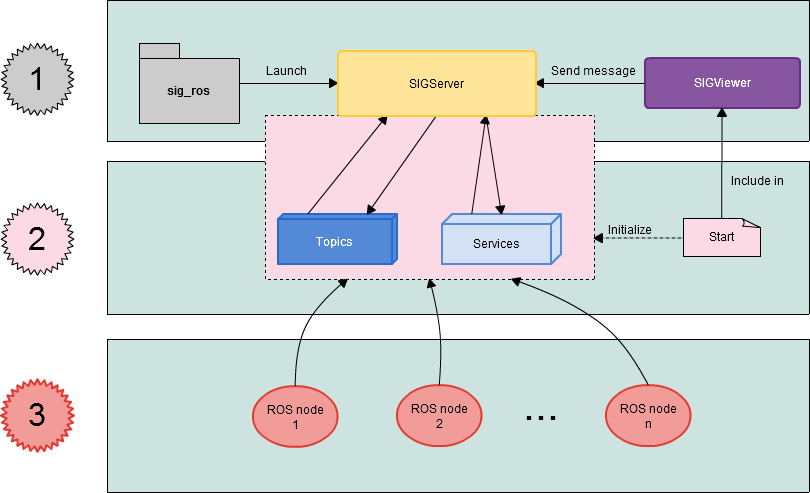
\includegraphics [width=150mm]{images/usage.png}}
\captionof{figure}{Steps to follow to start a simulation with ROS}\label{fig:usage}%      only if needed  
\end{minipage}

An example of the usage is here \url{https://www.youtube.com/watch?v=yskcDONc2CE&feature=youtu.be}. The video starts after the node ``ros\_controller'' has been launched. We can see the simulation starting, the topics and services are created, and the robot description of Hiro is loaded. After that, messages are launched from a terminal to different topics. The service of the inverse kinematics (see section \ref{subsec:ik}) is also called.

\section{Topics \& Services}
\subsection{Generalities}
Topics and services have to be defined. A node which subscribe to a topic receive the message as soon as it is published to the topic but no answer is given.\\
On the contrary, the service is a topic but it anwsers to the node who called the service.\\
The types of messages or service request can be of several simple type (double, string, ...) or a combination of these type or message created by these types.\\
It is possible to create new types, so the tranfert of SIGVerse object could be possible, but the use of the package has to be as easy as possible. So, the methods needed by the clean up task which return bad type for a message are replaced by a topic or service which execute a group of action, for exemple getPart and getPosition applied to the part are mixed in getPartPosition and the user only has to ask for a part and the position is returned with simple type ``double''.\\

The first step is to make the example of the clean up task working, so many topics and services have been created. Each of them starts by the name of the agent and follow by the name of the topic/service.

Now, we are going to see the topics and services I implemented for the robot agent, but a more exhaustive list with more details is given in annex~\ref{annex:topics} and annex~\ref{annex:services}. In those annexes, there are the topics for the robot agent but also for the object agent of the clean up task which I have started implementing.\\
The complete list of the topics, services, messages and services types is given in the user manual.

\subsection{Topics}
The list of the topics needed for the robot agent of the clean up task is:
\begin{description}
	\item[\_onRecvMsg] : The ``Controller'' send the message received by the SIGViewer.
	\item[\_onCollisionMsg] : The name of the agent which one is in collision with are sent to this topic. If there is severals collision at the same time, severals messages are sent.
	\item[\_setWheel] : Publish the radius and the distance in a message and they will be applied to the robot.
	\item[\_setWheelVelocity] : Publish the velocity for the left and the right wheel and it will be applied.
	\item[\_setJointVelocity] : set the velocity ``angular velocity'' to the join called ``jointName''.
	\item[\_releaseObj]: Publish the part which you want to release an object and it will be done.
\end{description}

The two first topics was obvious, they are the unique topics where the ``Controller'' publish. Indeed, the dynamic of the ``Controller'' run two methods when particular events occurs, see section~\ref{sec:controller}. That is why, each time it occurs, messages are sent to this topics.

\subsection{Services}
The list of the services needed for the robot agent of the clean up task is:
\begin{description}
	\item[\_get\_time] : Get the simulation time.
	\item[\_get\_obj\_position] : Get the position of the object named name, if name is empty, return the position of the agent which the service's name start with.
	\item[\_get\_parts\_position] : Get the position of the part in parameter.
	\item[\_get\_rotation] : Get the quaternion of the agent's rotation.
	\item[\_get\_angle\_rotation] : Get the angle of the rotation of the agent.
	\item[\_get\_joint\_angle]: Get the angle between the joint.
	\item[\_grasp\_obj]: Grasp the object ``obj'' with the part ``part''.
\end{description}


\section{SIGViewer service}
SIGViewer give a graphic interface for the visualization of the world and the robot. But many services can be connected to SIGViewer for example the referee of the Robocup competition.\\
The connection with the service is made at the SIGViewer level as we can see figure~\ref{fig:referee}. The user only has to install the service and add it to the SIGViewer. After that, the interaction with the service from the SIGServer is possible. Indeed, SIGServer is connected to the SIGViewer and the SIGViewer with the service.\\
Server side, the controller just need to send a message to the SIGViewer to connect with the service. After that, the controller can send every messages wanted to the service.\\

\noindent\begin{minipage}{\linewidth}% to keep image and caption on one page
\makebox[\linewidth]{%        to center the image
  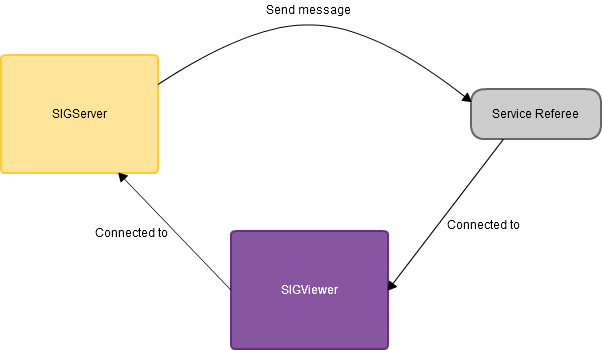
\includegraphics [width=150mm]{images/referee.png}}
\captionof{figure}{Links between SIGServer, SIGViewer and the referee service}\label{fig:referee}%      only if needed  
\end{minipage}

Basically, only few methods are related to the SIGViewer service, one for the connection, another for checking the connection and a last one for sending messages to the service. That is why I created two services ros more and one topic. With that, the user can connect all services he wants and interact with them.

\section{RoboCup Clean up task example}
The RoboCup clean up task aim to find the trash, take it and bring it to the good trashbox. We can see an example here \url{https://www.dropbox.com/sh/wwemhfzyg3rc5c6/AADqz8a0oEoK8hXK6uw1C48_a/SingleCleanUpDemo2014.wmv?dl=0}.\\
In this demonstration, two trashes are presents and the robot goes to each trash to bring it to a trashbox. Its actions are decided by a script. If a collision occurs points are taken off, if a good things happen points are given.\\
The count of the score is made by the referee service but a message is sent by a controller called ``Moderator'' to notify the referee.\\
The clean up task was the principal use case of the suggested work. We can see at \url{https://www.youtube.com/watch?v=Fc38tqwr0F0&feature=youtu.be} the result achieved.\\
We can notice that both videos are similar, that means the principal objective is accomplished.\\

In this second video, the actions of the robot are decided by a script, but this one is one or severals ros nodes who send messages to SIGVerse and get the robot moving as we can see figure~\ref{fig:cleanUpNodes}.\\

\noindent\begin{minipage}{\linewidth}% to keep image and caption on one page
\makebox[\linewidth]{%        to center the image
  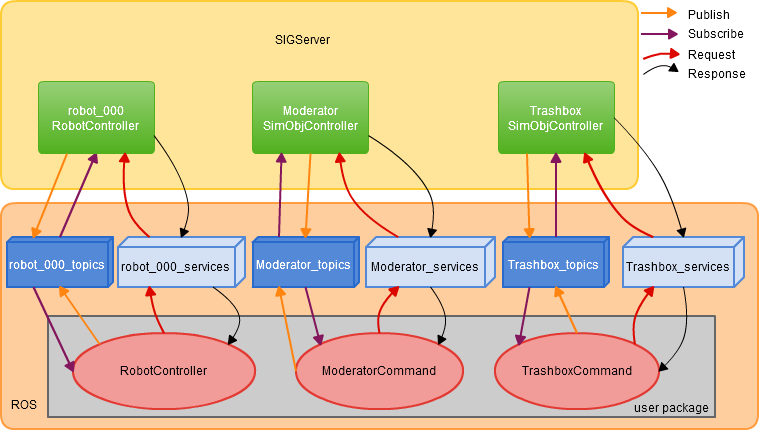
\includegraphics [width=150mm]{images/cleanUpNodes.png}}
\captionof{figure}{Controllers and nodes necessary to the Clean up task}\label{fig:cleanUpNodes}%      only if needed  
\end{minipage}

Three ``Controller'' are generated ``robot\_000'', ``Moderator'' and ``Trashbox'', with them the topics and services for each. By default, the name of the topics and services begins by the name of the ``Controller''.\\
Each script are inside three nodes: RobotCommand, ModeratorCommand and TrashboxCommand. It is the user part, he can program everything he wants to send messages to SIGServer. In this case, ``ModeratorCommand'' connects with the ``Referee'' service and send it messages, we can see the result on the left top corner in the video.\\
This is an easy example for the clean up task who can be find on the ``user'' package provided in the same repository as ``sig\_ros''.\\

Now, it is necessary to make this package capable of doing every movement for the robot, not only the clean up task. That is why just a mapping of every methods of SIGVerse to manipulate object and robot is necessary.\\
All topics and services availables are described in annex~\ref{annex:topics} and \ref{annex:services}.\\
A user manual is also available on the sig\_ros repository inside the doc folder of the sig\_ros package. This manual explains how to use the sig\_ros package and the example of the Clean up task.

\section{ROS package adapation}
\subsection{SLAM}
\subsubsection{Concept}\label{sec:slam_functionning}
The node SLAM take as entry two topics, /scan and /tf as we can see figure~\ref{fig:slam}. On the /scan topic, the information of the laser scan has to be published there. The type of the message is sensor\_msgs/LaserScan and the description can be found on \url{http://docs.ros.org/api/sensor_msgs/html/msg/LaserScan.html}. The ranges are the values of the distance between the robot and the next obtacle for each angle from angle\_min to angle\_max separated by angle\_increment on the positive way.\\
The range\_min and range\_max are respectively the min value and the max value possible for the range.\\
The intensity is not mandatory, it is the value for the obtacle transparence for the measurement.\\

The node subscribe to /tf too. /tf provide the tree of the robot from odometry to the laser place. That is why the minimum tree is /odom $\rightarrow$ /base\_link. Slam node also need /map $\rightarrow$ /odom but it provides it itself publishing to /tf.

The node publish to two topics and one service is available to get the map.\\

\noindent\begin{minipage}{\linewidth}% to keep image and caption on one page
\makebox[\linewidth]{%        to center the image
  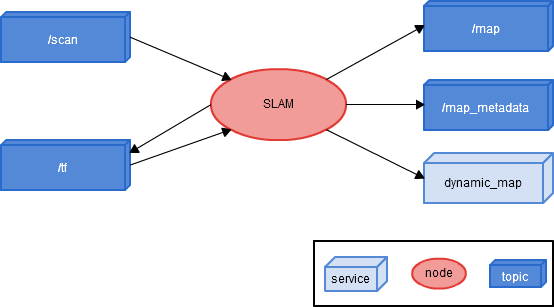
\includegraphics [width=150mm]{images/slam.png}}
\captionof{figure}{SLAM topics and services}\label{fig:slam}%      only if needed  
\end{minipage}

\subsubsection{Integration into SIGVerse}
As we saw section~\ref{sec:slam_functionning}, the topic scan and tf have to be published regularly. That is why the ``action'' will publish to the topics, because it is always called.\\
SIGVerse provide a laser scan for its robots, so the data only has to be modified to be on the /scan format.
For /tf, it is the same, but the tree has to be built depending on the robot. As the robot can be very different, I chose to build the easiest tree possible and assume that the laser scan is placed at the base\_link.\\

However, many problems occured due to a lack of documentation of the package. Indeed, the ros tutorial to use this package only explains the topics published and subscribed, services availables, parameters, and the type of the messages needed. But nothing about the meaning of the data needed. For example, the field ``range'' of the scan message has the description ``range data [m] (Note: values $<$ range\_min or $>$ range\_max should be discarded)'' but nothing says how the values are taken positive way, negative way, from 0 radian, from 90,...\\

There is two way to publish a message, publishing directly to a topic or send it by broadcast. /tf has to be sent by broadcast, but nothing informs the user.\\

Before the integration of this package to SIGVerse, I tried to use it with the turtlebot\footnote{Turtlebot is a low-cost, personal robot kit with open-source software used by ROS} simulator, it worked, I could move the turtlebot robot and the map was built. The same has to be done with SIGVerse simulator but no documentation exists about how turtlebot simulator publish information to make the slam package worked.

After many try, I decided to publish the information necessary to the SLAM package to two topics, then if the user wants to use SLAM, he can have access to the data and use it.

\subsection{Inverse kinematics}\label{subsec:ik}
\subsubsection{Concept}
ROS provide a package for solving the inverse kinematics and an example is provided on the documentation with a robot called pr2\footnote{The PR2 is a mobile manipulation platform built by Willow Garage. The PR2 software system is written entirely in ROS. As such, all pr2 capabilities are available via ROS interfaces.}. We can show pr2 with rviz\footnote{rviz is an 3D visualization tool for ROS} and launch a node from the tutorial to make move the robot in rviz using the inverse kinematics.\\
With this example, I was able to distinguish three parts of the work to realize, how the inverse kinematics package knows the description of pr2, how the information are sent to the ik package and how the result of the ik package is performed by rviz to make the robot moving. 

\subsubsection{Robot definition}
The ik package need two files, an urdf\footnote{Unified Robot Description Format} file to provide the description of the robot or an xacro file who generate the urdf file and a srdf\footnote{Semantic Robot Description Format} file which describe the semantic of the urdf file.\\

The SIGVerse robot is not the same as pr2, that is why the construction of an urdf file was necessary. Inside SIGVerse, the robot is described by an xml file which include non-standards x3d\footnote{A royalty-free ISO standard XML-based file format for representing 3D computer graphics} files. So, the transformation from x3d to urdf was not a good idea.\\
The best way was just modifying the urdf file of pr2 to look like the SIGVerse's robot.\\

The original urdf file had more than 4 000 lines, including ``transformation'' and gazebo tags. This two kind of tags are used by gazebo to make the robot moving easily, but inside SIGVerse, we do not need it, so the first step was to get rid of this tags.\\
Then, the urdf file is only made by ``link'' and ``joint'' tags. The structure of the file can be see as a tree starting by ``base\_link'' and putting a link between two joints. The origin of the child link of a joint make the length of its. We can see annex~\ref{annex:pr2Tree}, thanks to a tree, the original pr2 structure in the urdf file. \\
The second step was get rid of everything that the ik package does not need, some joints and links. At the same time, updating the srdf file removing the joints and links who are not necessary. The minimal structure of the robot can be see annex~\ref{annex:minStruct} \\
After that, it was just necessary to modify the size of the robot, height and arm's length related to the joints and links. For that I made a python script who modifies the length of the arms and the size of the robot of the file previously obtained.\\
Thanks to this script, the urdf file can be generated with the SIGVerse data. The robot can be changed just modifying the xml file for SIGVerse and if the robot has the same structure, the urdf file will be generated and the ik package will work as usual. The unique requirement is that the robot need the same structure.\\ 

Once the description file of the SIGVerse robot is built, it just need to fill the variable ``robot\_description'' of the ros launch file with the urdf file and the srdf file to make sure the ik package can access to the robot description.\\

\begin{figure}[h]
\centering
\begin{subfigure}{.5\textwidth}
  \centering
  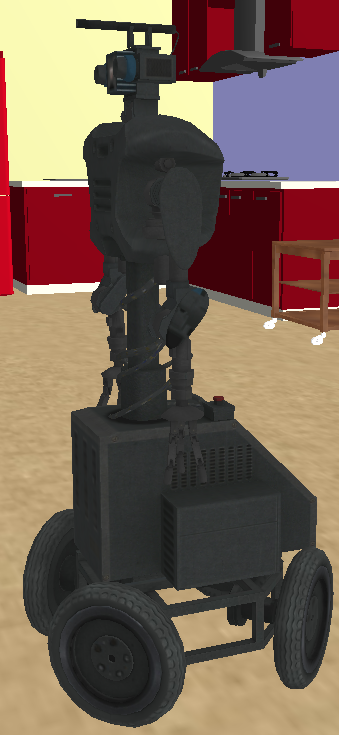
\includegraphics[width=50mm]{images/robot_000_sigverse.png}
  \caption{robot\_000 inside SIGVerse}
  \label{fig:robotSig}
\end{subfigure}%
\begin{subfigure}{.5\textwidth}
  \centering
  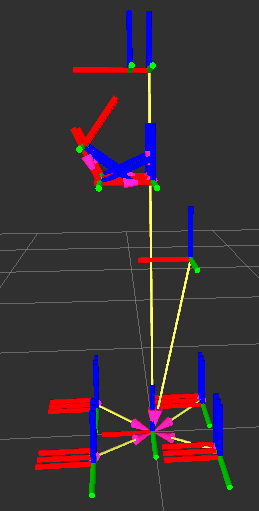
\includegraphics[width=55mm]{images/robot_000_rviz.png}
  \caption{robot\_000 described by urdf file}
  \label{fig:robotRviz}
\end{subfigure}
\caption{Visualisation of robot\_000}
\label{fig:robotVisu}
\end{figure}

We can see figure~\ref{fig:robotVisu}, the subfigure~\ref{fig:robotSig} shows the robot in the initial position inside SIGVerse and subfigure~\ref{fig:robotRviz} the same robot described by the urdf file viewed thanks to RViz. The robots have the same proportion but one difference is obvious, the position of the arms is not the same. A solution to this problem is explained section~\ref{subsubsec:integIKSIG}.\\
Between these two robots, another difference can be noticed, the orientation of the axis, indeed in SIGVerse y axis is vertical and x and z on the floor whereas in rviz, z is vertical.

\subsubsection{Result interpretation}
Once the ik package called, it answers a list of numbers corresponding to a list of joints names. The numbers are the angle in radian between the two links of a joint as we can see figure~\ref{fig:ikAngles}.
We can see the original position of the arm in red (it is the one showed in figure~\ref{fig:robotRviz}), the shoulder to the elbow measures 4 and the elbow to the wrist measures 3.21.\\
Then, if we ask for the position (0,1,0), the angle for the Elbow' is -0.813847 rad, that is why $\widehat{G,Elbow',Wrist'}$ = -46.63°.\\
For the shoulder, the angle with the original position and the new one will be -0.27157 rad for the position (0,1,0) and 0.23841 rad for the position (0,-1,0). The shoulder has 0 rad on its original position, indeed, we can see shoulderPan, shoulderLift and Elbow in the same line.

\noindent\begin{minipage}{\linewidth}% to keep image and caption on one page
\makebox[\linewidth]{%        to center the image
  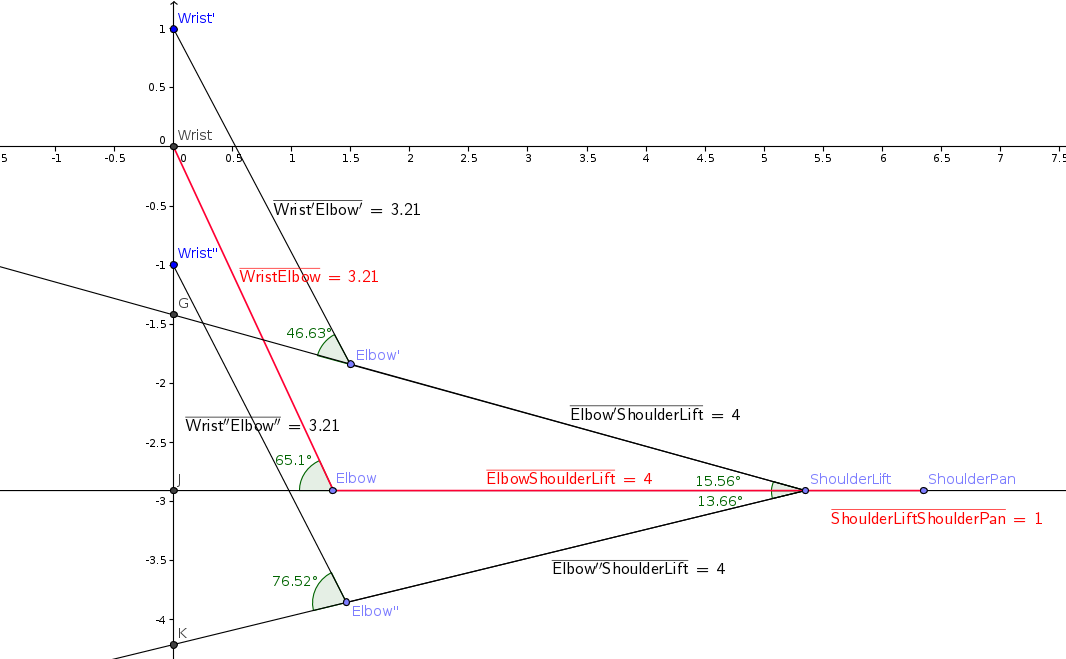
\includegraphics [width=150mm]{images/ggbAngles.png}}
\captionof{figure}{Angles between joints}\label{fig:ikAngles}%      only if needed  
\end{minipage}

\subsubsection{Integration into SIGVerse}\label{subsubsec:integIKSIG}
The ik package can figure out the position of every joint or not if the position of the end effector can not be reached. That is why I made a service, called ``\_ik'', available to use this package. The necessary data are simple, the position of the end effector hoped, the arm (left or right) whom the user wants to move and a last argument to provide the signification of the position.\\

We can see figure~\ref{fig:ikServ}, the concept for the use of the ik package is the same as a direct interaction with a robot (or object) inside SIGVerse. A service (ik) has to be called and the node RobotController will ask the ik package for the angles of each joints. After that, the RobotController interprets the result and make the arms of the SIGVerse robot moving.\\
The response by the service is necessary to notify the user node if the move has been possible (and so done) or not.

\noindent\begin{minipage}{\linewidth}% to keep image and caption on one page
\makebox[\linewidth]{%        to center the image
  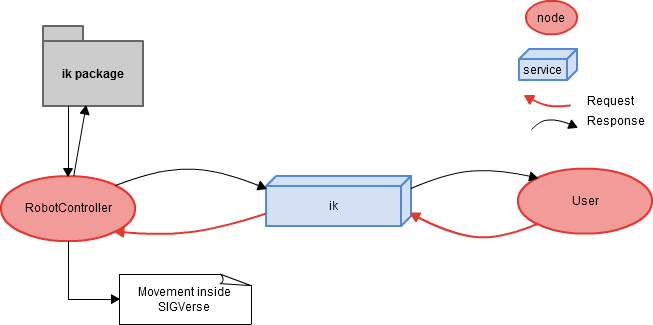
\includegraphics [width=150mm]{images/ik.png}}
\captionof{figure}{Architecture for the use of ik package}\label{fig:ikServ}%      only if needed  
\end{minipage}

The data position can be provided by three different form, absolute, relative or empty.\\
The empty form corresponds to the vector from the original position (0,0,0) and the new position.\\
The absolute position corresponds to the coordinates of SIGVerse where the user wants the arm to be.\\
The relative position corresponds to the vector from the current position to the new position.\\

The empty position does not need any treatment of the position given but the absolute and relative need to be modifyied. Indeed, the ik package need the data as the ``empty'' position, example figure~\ref{fig:ikAngles} the position (0,0,0) is the default position.\\
That is why, it was necessary to know the coordinate of the default position for calculate the vector from the default position to the wanted position. For that, I decided to apply matrix transformation to the arm hands position called ``Wrist''. See figure~\ref{fig:armCalculPoint} a visual of the problem.\\

The unit of the robot inside the urdf file is meter whereas inside SIGVerse it is the centimeter. Also, a little difference of scale can be found, so I took the position of few points see annex~\ref{annex:dataPos} and I calculated the average scale.\\
So, between the RobotController and the ``ik'' package in the figure~\ref{fig:ikServ} there is a little ``translator'' from SIGVerse position to urdf position.

\noindent\begin{minipage}{\linewidth}% to keep image and caption on one page
\makebox[\linewidth]{%        to center the image
  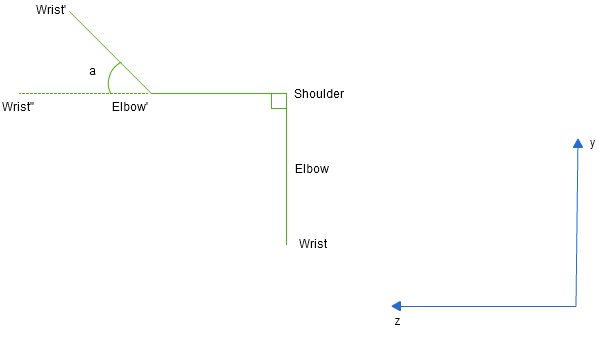
\includegraphics [width=130mm]{images/armCalculPoint.png}}
\captionof{figure}{Difference between the position of the arm in SIGVerse and RViz}\label{fig:armCalculPoint}%      only if needed  
\end{minipage}

In blue, we can see the axis of SIGVerse. The straight line Shoulder-Elbow-Wrist represents the initial position of the arm inside SIGVerse and the straight lines Shoulder-Elbow'-Wrist' the initial (default) position inside RViz.\\

The length of each part can be found thanks to SIGVerse and the angle ``a'' thanks to the ik package. Indeed, if we ask for the position (0,0,0) the angle ``a'' will be answered.\\
The computation of the points Elbow' and Wrist'' are easy, it is just the rotation of the original arm by 90 degrees around the point ``Shoulder'' and a rotation around the point ``Elbow''' of ``Wrist'''' with the angle ``a''.\\
For the point Wrist'', I used matrix of transformation as follow:\\
Wrist'' = T$_{-Shoulder}$ R$_{-90}$ T$_{Shoulder}$ Wrist\\
For the point Elbow':\\
Elbow' = T$_{-Shoulder}$ R$_{-90}$ T$_{Shoulder}$ Elbow\\
For the point Wrist':\\
Wrist' = T$_{-Elbow'}$ R$_{-a}$ T$_{Elbow'}$ Wrist'' with:\\

T$_{P}$ =
$\begin{pmatrix}
   1 & 0 & 0 & P_x \\
   0 & 1 & 0 & P_y \\
   0 & 0 & 1 & P_z \\
   0 & 0 & 0 & 1
\end{pmatrix}$ and 
R$_{\theta}$ = 
$\begin{pmatrix}
   1 & 0 & 0 & 0 \\
   0 & cos(\theta) & -sin(\theta) & 0 \\
   0 & sin(\theta) & cos(\theta) & 0 \\
   0 & 0 & 0 & 1
\end{pmatrix}$

This computation is made for both arms. This, allows the user to not having a symetric robot, he can decide of the length of each part independently.

\section{Internship progress}
\subsection{Discovery}
The first two weeks were dedicated to the installation of the environment: Operating System, Virtual Machine, SIGServer, SIGViewer. After that, I could see how SIGVerse works. 

Ones the environment installed, I was able to run examples of the wiki page \cite{SIGVerseWiki}. With this examples, I could see the function of the ``Controller'' and then understand how an agent can act, changing places, saying ``Hello'',... But also, how an agent communicates in both ways, sending and receiving messages.\\

After installing the environment and learning how to create an agents and make them move, I had to know what was ROS and how it is working. So, I installed all the environment and I did the tutorials of the wiki page \cite{ROSWiki}.\\
After that, I could run an example of SIGVerse running with ROS and then beginning to investigate how to design an interface between SIGVerse and ROS.

\subsection{Tools}
At the beginning, I was developping on a virtual machine Ubuntu 12.04, but few weeks later SIGVerse was officially available on Ubuntu 14.04, the stablest version where SIGVerse works well. Because of many troubles on Ubuntu 12.04, I decided to upgrade to Ubuntu 14.04.\\
No IDE\footnote{Integrated Development Environment} is used, only a text editor gedit and a terminal for compilation. ROS and SIGVerse are open source so, I decided to use GitHub.\\
Because of the reinstallation of the virtual machine, a behaviour was not expected, un keyboard problem, so I decided to change my text editor to vim\footnote{Visual Interface IMproved}.\\ 
I am using Windows 8.1 for the compatibility with the kinect which I could need during the project.\\

I used Geogebra software to verify my theories about the angles answered by the inverse kinematics package.\\
I used Cacoo on line to make every schema of this report.\\
I make unit tests with ROS to be sure of the good functioning.

\subsection{Organisation}
The choice of my subject was very open, my supervisor showed me the simulator SIGVerse and the first step after the installation was finding a subject. Because of the short time due to the DoW\footnote{Description of Work} deadline, I chose to work on this project.\\
After the three first months, the main part was done, that means the Clean up task demo and the development of topics and services necessary to have a full access to SIGVerse functionnalities from ROS.\\
After that, I started to add functionnalities to my package. This new functionnalities are an adaptation of the use of a ROS package to SIGVerse. I included the SLAM and inverse kinematics package.\\

Once a week, all laboratory's members attends a meeting where each members exposes what he planned to do the week before, what he actually did and what he will do the next week. I make my own objectives every week for achieving the main goal.\\
My supervisor answers to my questions and gives me indications during the meeting.

\subsection{Troubles}
\subsubsection{Development}
First of all, due to my lack of knowledge about ROS, it was very difficult to gain a full view of the project at the beginning. That is why, I had to spend some days to learn from the ROS tutorials and to practice with this framework.\\
When I started implementing the ``Controller'', I had a problem of inheritance. Indeed, I had to inherit the robot ``Controller'' from the object ``Controller'' and keep this two ``Controller'' usable for an agent. This inheritance was not easy because of ROS.\\
I found SIGVerse bug using a function ``getSimulationTime()'' and others functions. I spent a lot of time diagnosing this bug because I though it came from my code but finally it was a SIGVerse error. So, I made a bug report.\\
Sometimes it is just the function who does not answer the good thing, sometimes if we put a wrong arguments, the all simulator can stop.

\subsubsection{Documentation}
The documentation of SIGVerse is in japanese, so it is quiet difficult to understand what every method does, so I did a lot of tests to figure it out. Fortunately, Google translate can be a good help.\\

For the adaptation of the package SLAM and inverse kinematics, we can find a lot of tutorials to use this packages but none of them explains how they works.\\
For example, we can find turtlebot and a simulator of its. Using the simulator Rviz, we can make the SLAM package works, the data send by turtlebot make possible the computation of the map. If I register the messages sent by turtlebot and then I send it from SIGVerse, it works, but if I make my own messages, it is not working. But no information can be found about this messages, just the structure but not the containt. So, I asked for the help of the community, posting a message on the forum.\\

For the inverse kinematics package, it is the same problem, there was no information neither the interpretation of the result nor how to set the description of the robot. I figured it out thanks to the examples, trying to understand how it was working.\\

Thanks to the rosdoc\_lite I could generate a technical documentation for my package.

\subsubsection{Conception}
The objective of this interface is increasing the number of SIGVerse users by adding ROS users. So, the use of my package has to be instinctive, so the choice of the topics and services has to be relevant.\\
I made the choice to add an argument to each topics or services called ``name'', this argument is the same for all of them, that means the object or robot to whom it is applyied.\\

For the inverse kinematics, I chose to make available three types of position: relative, absolute and respect to the ``default'' position.\\
The computation of the default position inside SIGVerse was not easy because of two centimeters less than I had to find. The source of this two centimeters issue was no obvious, it can be because of the robot description, the computation itself or SIGVerse. But this issue is quit important because if the user ask for example for the position (116.64, 85, 42), the inverse kinematics package will answer it not find a solution because the computation of the default position is (116.64, 90, 40) and not (116.64, 90, 42), so my package will ask for the vector (0, -5, 2) instead of (0, -5, 0).

\subsection{Schedule}
\subsubsection{What I planned}
In the DoW report, I planned to achieve the job L2 before the mid-term report deadline. That means make SIGVerse works with ROS by a simple way like one ``Controller'' with one node and generate a ``Controller'' for each agent on the simulator.\\

After that, I planned to design and develop the topics and services that are necessary to control the agents. I also planned to make an interface between the real human and the simulator. For example, making work the kinect. We can see annex~\ref{GanttChart} the schedule of the DoW.

\subsubsection{What I actually did}
Finally, the first part (before de mid-term report about making work a simple ``Controller'' with one node) was easier than I though and I could start the next job. So, I started implementing some topics and services for the clean up task before the mid-term report.\\
Only the methods for the clean up task have been done and some others. You can see at \url{https://www.youtube.com/watch?v=PL4MCjire2M&feature=youtu.be} a demonstration of the clean up task. The actions of the robot are sent by ROS.\\

After that, I finished to develop the others topics and services for an all control of the robot. Then, I dealt with the referee during one month.\\
At this point, a demonstration was possible at a weekly meeting, the video of it is available here \url{https://www.youtube.com/watch?v=Fc38tqwr0F0&feature=youtu.be}. We can see the robot going for the trash and the referee at the left top corner counting the points.

Then, 3 months left so I decided to make more tests and I found bug on my package and on SIGVerse. After that, I made an adaptation of two ROS package who can provide more functionnalities to SIGVerse.\\
We can see figure~\ref{GanttChart:final} the schedule who actually occured.

\subsubsection{Reason of the changement}
The first changement has been made because it was easier than I though, but then, the second part has been changed because it was more interesting to add functionnalities to SIGVerse than adding the kinect.\\
Indeed, SLAM and inverse kinematics are two useful tools for every user, not only for those who use the kinect.

\subsubsection{To continue}
First of all, we can notice that the user need to modify every link inside the sig\_ros package in order to link ROS to SIGServer and to link the controller to the objects and robots. Once the relatives links will be allowed by SIGVerse, these modifications by the user will not be useful and the package will be able to use easier.\\
The inverse kinematics is very useful, but in this case, the functionnality only works with the robot hiro and the variation of the size of this robot. The best would be adapting the initialisation of the ik package to any kind of robot only with SIGVerse information available.\\
For the SLAM package, of course integrating it completely, not only sending the information necessary would be better.


\begin{landscape}
%\subsection{Schedule}\label{sec:schedule}
%\thispagestyle{empty}
%\thispagestyle{plain}
\setlength{\topmargin}{25pt}
\titlespacing{\subsection}{0cm}{0cm}{0cm}


\noindent\begin{ganttchart}[
hgrid,
vgrid,% = {*6{white}, *1{black}},% *{10}{blue, dashed}},
x unit=0.3cm,
%title/.style={fill=teal, draw=none},
%title label font=
%\color
%{white}
%\bfseries,
inline,
time slot format=isodate,
]{2015-03-16}{2015-06-07}
\gantttitlecalendar{year, month=name, week}{4} \\
\ganttbar{Planification}{2015-03-16}{2015-04-12}
\ganttbar{Project monitoring}{2015-04-13}{2015-06-07}\\

\ganttbar{DoW Report}{2015-04-03}{2015-04-12}
\ganttbar{Environment installation}{2015-03-16}{2015-03-28}
\ganttbar{Tutorials}{2015-03-29}{2015-04-02}
\ganttbar{L2:T1}{2015-04-13}{2015-04-19}
\ganttmilestone{DoW}{2015-04-12}
\ganttbar{L2:T2}{2015-04-20}{2015-05-03}
\ganttbar{L2:T3}{2015-05-04}{2015-05-10}
\ganttbar{Topics \& Services}{2015-05-18}{2015-05-31}
\ganttbar{Referee Service}{2015-06-01}{2015-06-07}\\

\ganttbar{Technical documentation}{2015-04-13}{2015-05-10}
\ganttbar{Technical documentation}{2015-05-18}{2015-06-07}\\

\ganttbar{Mid-term Report}{2015-05-04}{2015-05-17}
\ganttmilestone{Mid-term report}{2015-05-17}

\end{ganttchart}

\noindent\begin{ganttchart}[
hgrid,
vgrid,
x unit=0.3cm,
inline,
time slot format=isodate,
]{2015-06-08}{2015-08-30}
\gantttitlecalendar{month=name, week = 13} \\
\ganttbar{Project monitoring}{2015-06-08}{2015-08-30}\\
\ganttbar{SLAM adaptation}{2015-06-08}{2015-06-28}
\ganttbar{Inverse Kinematics}{2015-06-29}{2015-07-27}
\ganttbar{Tests}{2015-07-28}{2015-08-02}
\ganttbar{Final Report}{2015-08-10}{2015-08-30}\ganttmilestone{Final Report}{2015-08-30}\\
\ganttbar{Technical documentation}{2015-06-08}{2015-08-02}
\ganttbar{User documentation}{2015-08-03}{2015-08-16}
\end{ganttchart}
\captionof{figure}{Real schedule of the internship}\label{GanttChart:final}
\end{landscape}

 

\chapter{Conclusion}
\setlength{\parskip}{2.5ex plus .4ex minus .4ex}
%1. Ce que le stage m'a apporté
%2. Logiciel fonctionnel..
%Ce qui reste, tests fonctionnel, de performance
These two first month of internship make me see a research environment: discovering a new project, finding a subject and designing a solution by myself.\\
I learnt a lot with the autonomy I had: designing, implementing, testing and finding a solution to the bugs who occured, but also technical skills like C++.\\

The interface I began to develop has to be functional by the end of the internship. Indeed, ROS users will use my package or may be SIGVerse users who thinks using ROS is an easier way to use SIGVerse. This objective of achievement is very motivated.\\

For the rest of the internship, many things have to be done, finishing the clean up task, testing, designing and developping the interaction human-SIGVerse.

%Grâce à ce stage, j'ai pu voir comment développer de nouvelles fonctionnalités à partir de besoins précisés en début de stage. Ces besoins s'attachaient à un logiciel existant, il a donc fallu apprendre à lire et comprendre le fonctionnement avant toute modification et/ou ajout de code.\\
%J'ai également pu voir plusieurs aspects de développement, créer un plugin sur un logiciel existant, créer les fonctionnalités de ce plugin, créer son interface graphique mais aussi l'aspect debuguage, rapport de bug du logiciel existant et debuguage de mon propre code.\\
%Ce stage m'a apporté des compétences telles que le moyen de répondre à un besoin, de rechercher des informations, mais aussi des compétences techniques notamment en C++.\\
%
%A la fin de ce stage, le plugin développé est fonctionnel, les usagés peuvent s'en servir afin de modéliser des individus dans le sens IBM.\\
%Ce plugin fournit de nouvelles possibilités que VLE ne pouvait pas offrir auparavant. Cependant, du travail reste à faire comme des tests sur les fonctionnalités. En effet, le plugin répond actuellement aux besoins cités en première partie mais peut-être que de nouveaux cas d'utilisation sont à venir et de nouvelles fonctionnalités seraient nécessaires comme par exemple faciliter l'inclusion de modèle IBM dans d'autres modèles, proposer à l'utilisateur une interface afin qu'il choisisse les ports d'entrée et de sortie qui lui sont nécessaire...\\
%De plus, certaines fonctionnalités comme l'observation de variable globale est possible mais aucune interface graphique n'a été développée.\\


\begin{thebibliography}{9}
\addcontentsline{toc}{chapter}{Bibliography}
	\bibitem{SIGVerseWiki}
          SIGVerse wiki page : 
          \url{http://www.sigverse.org/wiki/en/index.php?Tutorial}.
	\bibitem{ROSWiki}
          ROS wiki page :
          \url{http://wiki.ros.org/fr/ROS/Tutorials}.
     \bibitem{SIGVerseWikiROS}
          SIGVerse wiki page ROS integration tutorial :
          \url{http://www.sigverse.org/wiki/en/index.php?ROS%20integration}.
     
\end{thebibliography}

\newpage 
\vspace*{\fill}
\begin{abstract}
\addcontentsline{toc}{chapter}{Abstract}
I did this internship in the National Institute of Informatics, an inter university research institute which aim to develop the research in multiple domains. But more specifically, in the Inamura lab.\\
My subject was making an interface between ROS and SIGVerse for growing the SIGVerse community. ROS is a framework for writing robot software and SIGVerse a simulator.\\
The interface is made in C++ and I tried to make it very easy for the ROS users. Their knowledge about SIGVerse can be very limited or totally inexistant. The ROS users will be able to use SIGVerse as easy as possible. They only have to publish or subscribe topics or to call services that I defined like any ROS package.\\
The developpement of this package allowed to include more fonctionnalities to SIGVerse from ROS like the inverse kinematics or SLAM.\\
This project made me very responsible and independant in the area of software design, need analysis...\\

J'ai réalisé ce stage dans le laboratoire d'Inamura, au National Institute of Informatics, un institut de recherche dans divers domaines.\\
Le but de ce projet est de créer une interface entre ROS et SIGVerse afin d'agrandir la communauté de SIGVerse.\\
ROS est un framework pour le développement de logiciel pour les robots et SIGVerse un simulateur.\\
L'interface est réalisée en C++ et son utilisation doit être la plus simple possible pour un utilisateur ROS, c'est-à-dire sans ou peu de connaissances de SIGVerse prérequises. Les utilisateurs ROS doivent être capable de communiquer avec SIGVerse sans difficultés, juste en publiant et/ou souscrivant à des ``topics'' ou appelant des services.\\
Le développement de ce package a permit l'ajout de fonctionnalités à SIGVerse. En effet, la cinématique inverse et SLAM peuvent maintenant être utilisé dans SIGVerse.\\
Ce projet m'a permis d'appliquer mes connaissances de manière responsable et autonome dans l'analyse des besoins, conception...
\end{abstract}
\vspace*{\fill}

\appendix
\chapter{Annex}
\setlength{\parskip}{2.5ex plus .4ex minus .4ex}
\section{Jobs}
\definecolor{cyan}{rgb}{0.7,0.7,1}
\noindent\begin{minipage}{\linewidth}% to keep image and caption on one page
\begin{center}
\begin{tabular}{| l | m{8cm} | c | c |}
\hline
	N & Title & Start & End\\\hline
	\rowcolor{cyan} L1 & Management & & \\
	T1	& Planning & S1 & S4\\
	T2	& Project monitoring & S5 & S24\\
	\rowcolor{cyan}L2 & SIGServer and agents integration & &\\
	T1	& Run SIGServer from ROS & S5 & S5\\
	T2	& Generation of one controller associated to one agent & S6 & S7\\
	T3	& Generation of controller for each agents & S8 & S8 \\
	\rowcolor{cyan}L3 & Make agents act & &\\
	T1	& Though Publish/Subscribe & S10 & S12\\
	T2	& Though ROS Services & S13 & S15\\
	\rowcolor{cyan}L4 & Services interface & &\\
	T1	& Design & S16 & S17\\
	T2	& Kinect & S18 & S20\\
	\rowcolor{cyan}L5 & Documentation & &\\
	T1	& Technical documentation & S5 & S18\\
	T2	& User documentation & S19& S23\\
	\rowcolor{cyan}L6 & Report & &\\
	T1	& Mid-term report & S8 & S9\\
	T2	& Final report & S22 & S24\\\hline
\end{tabular}
\end{center}
\captionof{table}{Jobs}\label{tab:lots}%      only if needed  
\end{minipage}

\begin{landscape}
\section{Schedule}\label{sec:schedule}
%\thispagestyle{empty}
%\thispagestyle{plain}
\setlength{\topmargin}{25pt}
\titlespacing{\subsection}{0cm}{0cm}{0cm}


\noindent\begin{ganttchart}[
hgrid,
vgrid,% = {*6{white}, *1{black}},% *{10}{blue, dashed}},
x unit=0.3cm,
%title/.style={fill=teal, draw=none},
%title label font=
%\color
%{white}
%\bfseries,
inline,
time slot format=isodate,
]{2015-03-16}{2015-06-07}
\gantttitlecalendar{year, month=name, week}{4} \\
\ganttbar{Planification}{2015-03-16}{2015-04-12}
\ganttbar{Project monitoring}{2015-04-13}{2015-06-07}\\

\ganttbar{DoW Report}{2015-04-03}{2015-04-12}
\ganttbar{Environment installation}{2015-03-16}{2015-03-28}
\ganttbar{Tutorials}{2015-03-29}{2015-04-02}
\ganttbar{L2:T1}{2015-04-13}{2015-04-19}
\ganttmilestone{DoW}{2015-04-12}
\ganttbar{L2:T2}{2015-04-20}{2015-05-03}
\ganttbar{L2:T3}{2015-05-04}{2015-05-10}
\ganttbar{L3:T1}{2015-05-18}{2015-06-07}\\

\ganttbar{Technical documentation}{2015-04-13}{2015-05-10}
\ganttbar{Technical documentation}{2015-05-18}{2015-06-07}\\

\ganttbar{Mid-term Report}{2015-05-04}{2015-05-17}
\ganttmilestone{Mid-term report}{2015-05-17}

\end{ganttchart}

\noindent\begin{ganttchart}[
hgrid,
vgrid,
x unit=0.3cm,
inline,
time slot format=isodate,
]{2015-06-08}{2015-08-30}
\gantttitlecalendar{month=name, week = 13} \\
\ganttbar{Project monitoring}{2015-06-08}{2015-08-30}\\
\ganttbar{L3:T2}{2015-06-08}{2015-06-28}
\ganttbar{L4:T1}{2015-06-29}{2015-07-12}
\ganttbar{L4:T2}{2015-07-13}{2015-08-02}
\ganttbar{Final Report}{2015-08-10}{2015-08-30}\ganttmilestone{Final Report}{2015-08-30}\\
\ganttbar{Technical documentation}{2015-06-08}{2015-08-02}
\ganttbar{User documentation}{2015-08-03}{2015-08-16}
\end{ganttchart}
\label{GanttChart}
\end{landscape}


\section{Topics}\label{annex:topics}
\begin{supertabular}{|p{2.9cm}|p{4.5cm}|p{7cm}|}
	\hline
    Topic name & Message & Description \\
  	\hline
  	\_onRecvMsg &
  		\textbf{sender} : string\newline 
  		\textbf{content} : string
  		\medskip & The ``Controller'' send the message received by the SIGViewer.\\
  	\hline
  	\medskip
  	\_onCollisionMsg &
  		\medskip
  		\textbf{name} : string \newline
  		\textbf{part} : string & The name of the agent which one is in collision with are sent to this topic. If there is severals collision at the same time, severals messages are sent.\\
  	\hline
  	\_setWheel & 
  		\textbf{wheelRadius} : double \newline
  		\textbf{wheelDistance} : double & Publish the radius and the distance in a message and they will be applied to the robot.\\
  	\hline
  	\_setWheelVelocity & 
  		\textbf{leftWheel} : double \newline
  		\textbf{rightWheel} : double
  		& Publish the velocity for the left and the right wheel and it will be applied.\\
  	\hline
  	\_setJointVelocity & 
  		\textbf{jointName} : string\newline
  		\textbf{angularVelocity} : double \newline
  		\textbf{max} : double
  		& jointName, angular velocity, max ???\\
  	\hline
  	\_releaseObj & \textbf{arm} : string & Publish the part which you want to release an object and it will be done.\\
  	\hline
  	\_setAxisAndAngle & 
  		\textbf{name} : string \newline
  		\textbf{axisX} : double \newline
  		\textbf{axisY} : double \newline
  		\textbf{axisZ} : double \newline
  		\textbf{angle} : double
  		& Set the axis defined by ``axisX'', ``axisY'' and ``axisZ'' and set the angle ``angle'' to the entity called ``name'', if no name is provided, the main entity of the topic will be set.\\
  	\hline
  	\_setPosition & 
  		\textbf{name} : string \newline
  		\textbf{posX} : double \newline
  		\textbf{posY} : double \newline
  		\textbf{posZ} : double
  		& Set the position ``posX'', ``posY'' and ``posZ'' to the entity called ``name'', if no name is provided, the main entity of the topic will be set.\\
  	\hline
\end{supertabular}

\section{Services}\label{annex:services}
\begin{supertabular}{|p{2.9cm}|p{2.5cm}|p{3cm}|p{5.5cm}|}
	\hline
    Service name & Request & Response & Description \\
  	\hline
  	\_get\_time &  & \textbf{time} : double & Get the simulation time.\\
  	\hline
  	\medskip
  	\_get\_obj\_position & \medskip \textbf{name} : string & 
  		\textbf{posX} : double \newline
  		\textbf{posY} : double \newline
  		\textbf{posZ} : double
  		 & Get the position of the object named name, if name is empty, return the position of the agent which the service's name start with.\\
  	\hline
  	\_get\_parts\_position & \textbf{part} : string & 
  		\begin{minipage}{3cm}
  			\medskip
  			\begin{description} 
  				\item[posX] : double 
  				\item[posY] : double 
  				\item[posZ] : double
  			\end{description}
  			\medskip
  		\end{minipage} & Get the position of the part in parameter.\\
  	\hline
  	\_get\_rotation & \textbf{axis} : string & 
  		\begin{minipage}{3cm}
  			\medskip
  			\begin{description} 
  				\item[qW] : double 
  				\item[qX] : double 
  				\item[qY] : double
  				\item[qZ] : double
  			\end{description}
  			\medskip
  		\end{minipage} & Get the rotation of ...\\
  	\hline
  	\_get\_angle\_rotation & 
  		\begin{minipage}{3cm}
  			\medskip
  			\begin{description} 
  				\item[axis] : string
  				\item[x] : double 
  				\item[y] : double 
  				\item[z] : double
  			\end{description}
  			\medskip
  		\end{minipage} & \textbf{angle} : double & Get the angle of ...\\
  	\hline
  	\_get\_joint\_angle & \textbf{nameArm} : string & \textbf{angle} : double & Get the angle between the joint.\\
  	\hline
  	\_grasp\_obj & 
  		\begin{minipage}{3cm}
  			\medskip
  			\begin{description} 
  				\item[part] : string
  				\item[obj] : string
  			\end{description}
  			\medskip
  		\end{minipage} & \textbf{ok} : bool & Grasp the object ``obj'' with the part ``part''\\
  	\hline
  	\_get\_entities & \textbf{axis} : string & 
  		\begin{minipage}{3cm}
  			\medskip
  			\begin{description} 
  				\item[entitiesNames] : string[] 
  				\item[length] : int
  			\end{description}
  			\medskip
  		\end{minipage} & Get the names of the entities in the simulator.\\
  	\hline
  	\_check\_service & \textbf{serviceName} : string & \textbf{connected} : bool & Check if the service ``serviceName'' is connected.\\
  	\hline
  	\_connect\_to\_service & \textbf{serviceName} : string & \textbf{connected} : bool & Connect the ``serviceName'', true if it is connected, false otherwise.\\
  	\hline
  	\_get\_collision\_state \_of\_main\_part & & \textbf{collisionState} : bool & Get the collision state of the main part.\\
  	\hline
  	\_is\_grasped & \textbf{entityName} : string & \textbf{answer} : bool & True if ``entityName'' is grasped, false otherwise. If no entity name is provided, it will return the answer for the agent which is asked\\
  	\hline
\end{supertabular}

%\section{pr2 tree}\label{annex:pr2Tree}
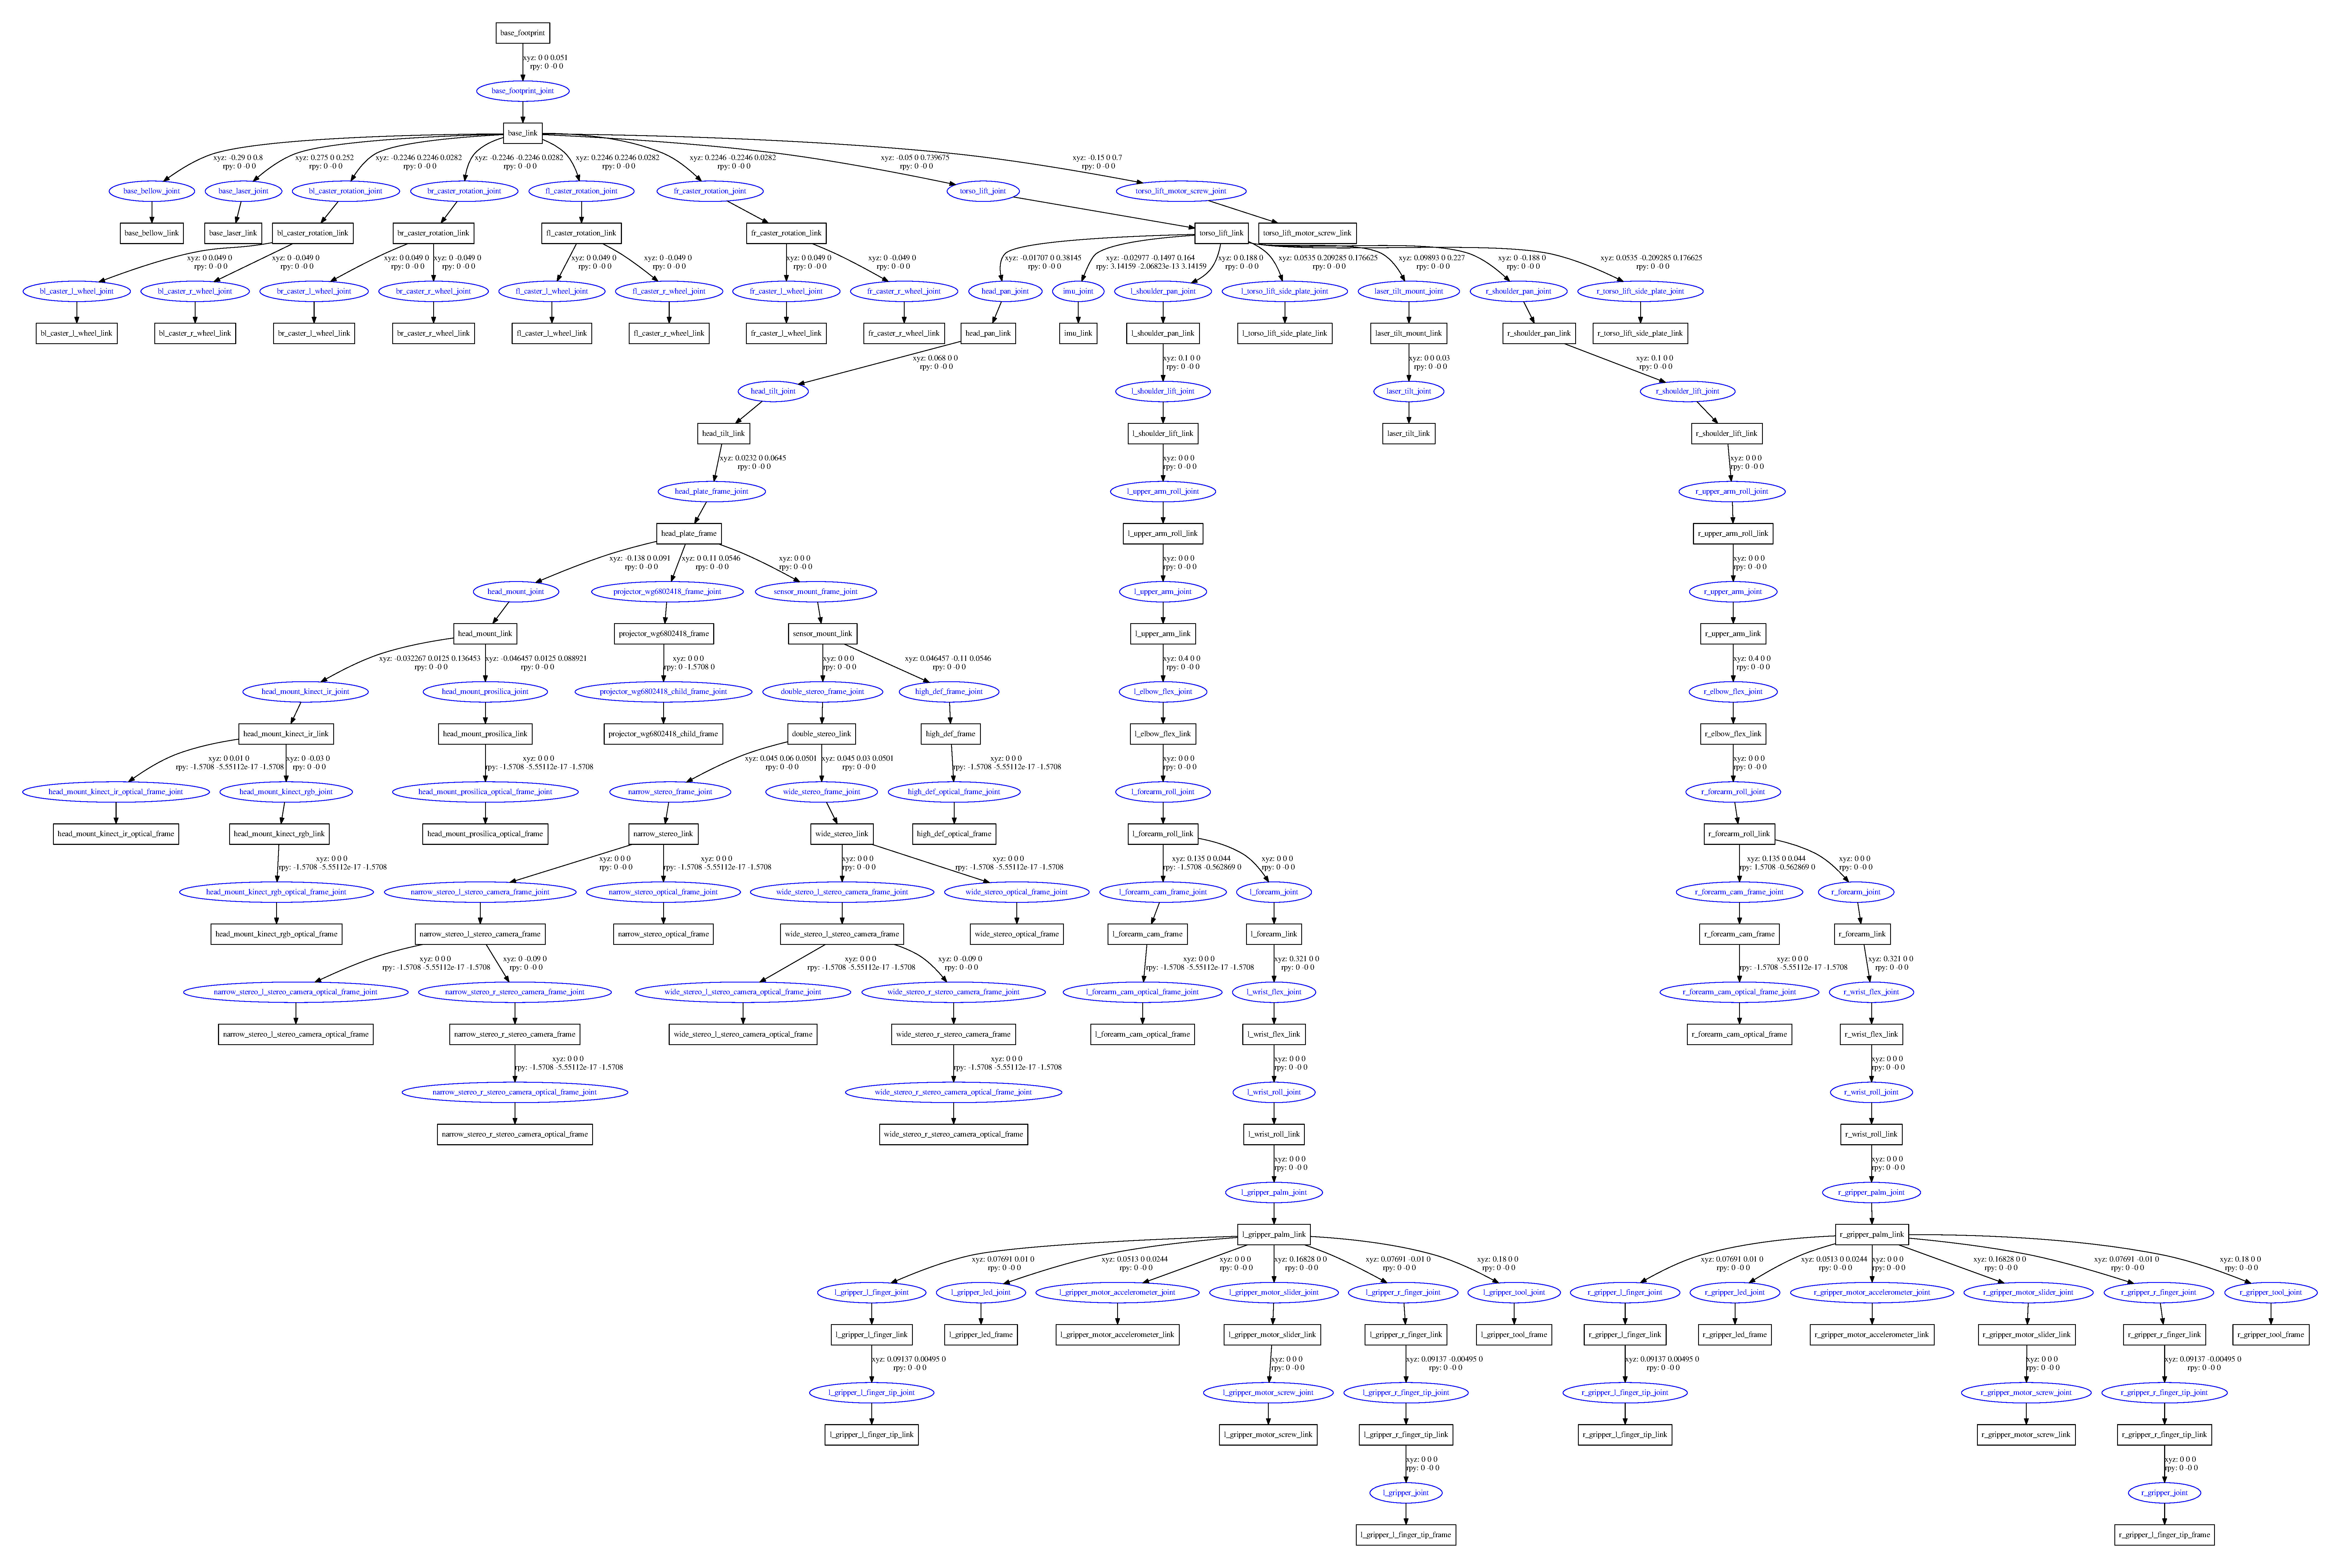
\includepdf[scale=0.95,pages=1,pagecommand=\section{Pr2 tree}\label{annex:pr2Tree}]{images/pr2Tree.pdf}
%\section{Minimal structure tree}\label{annex:minStruct}
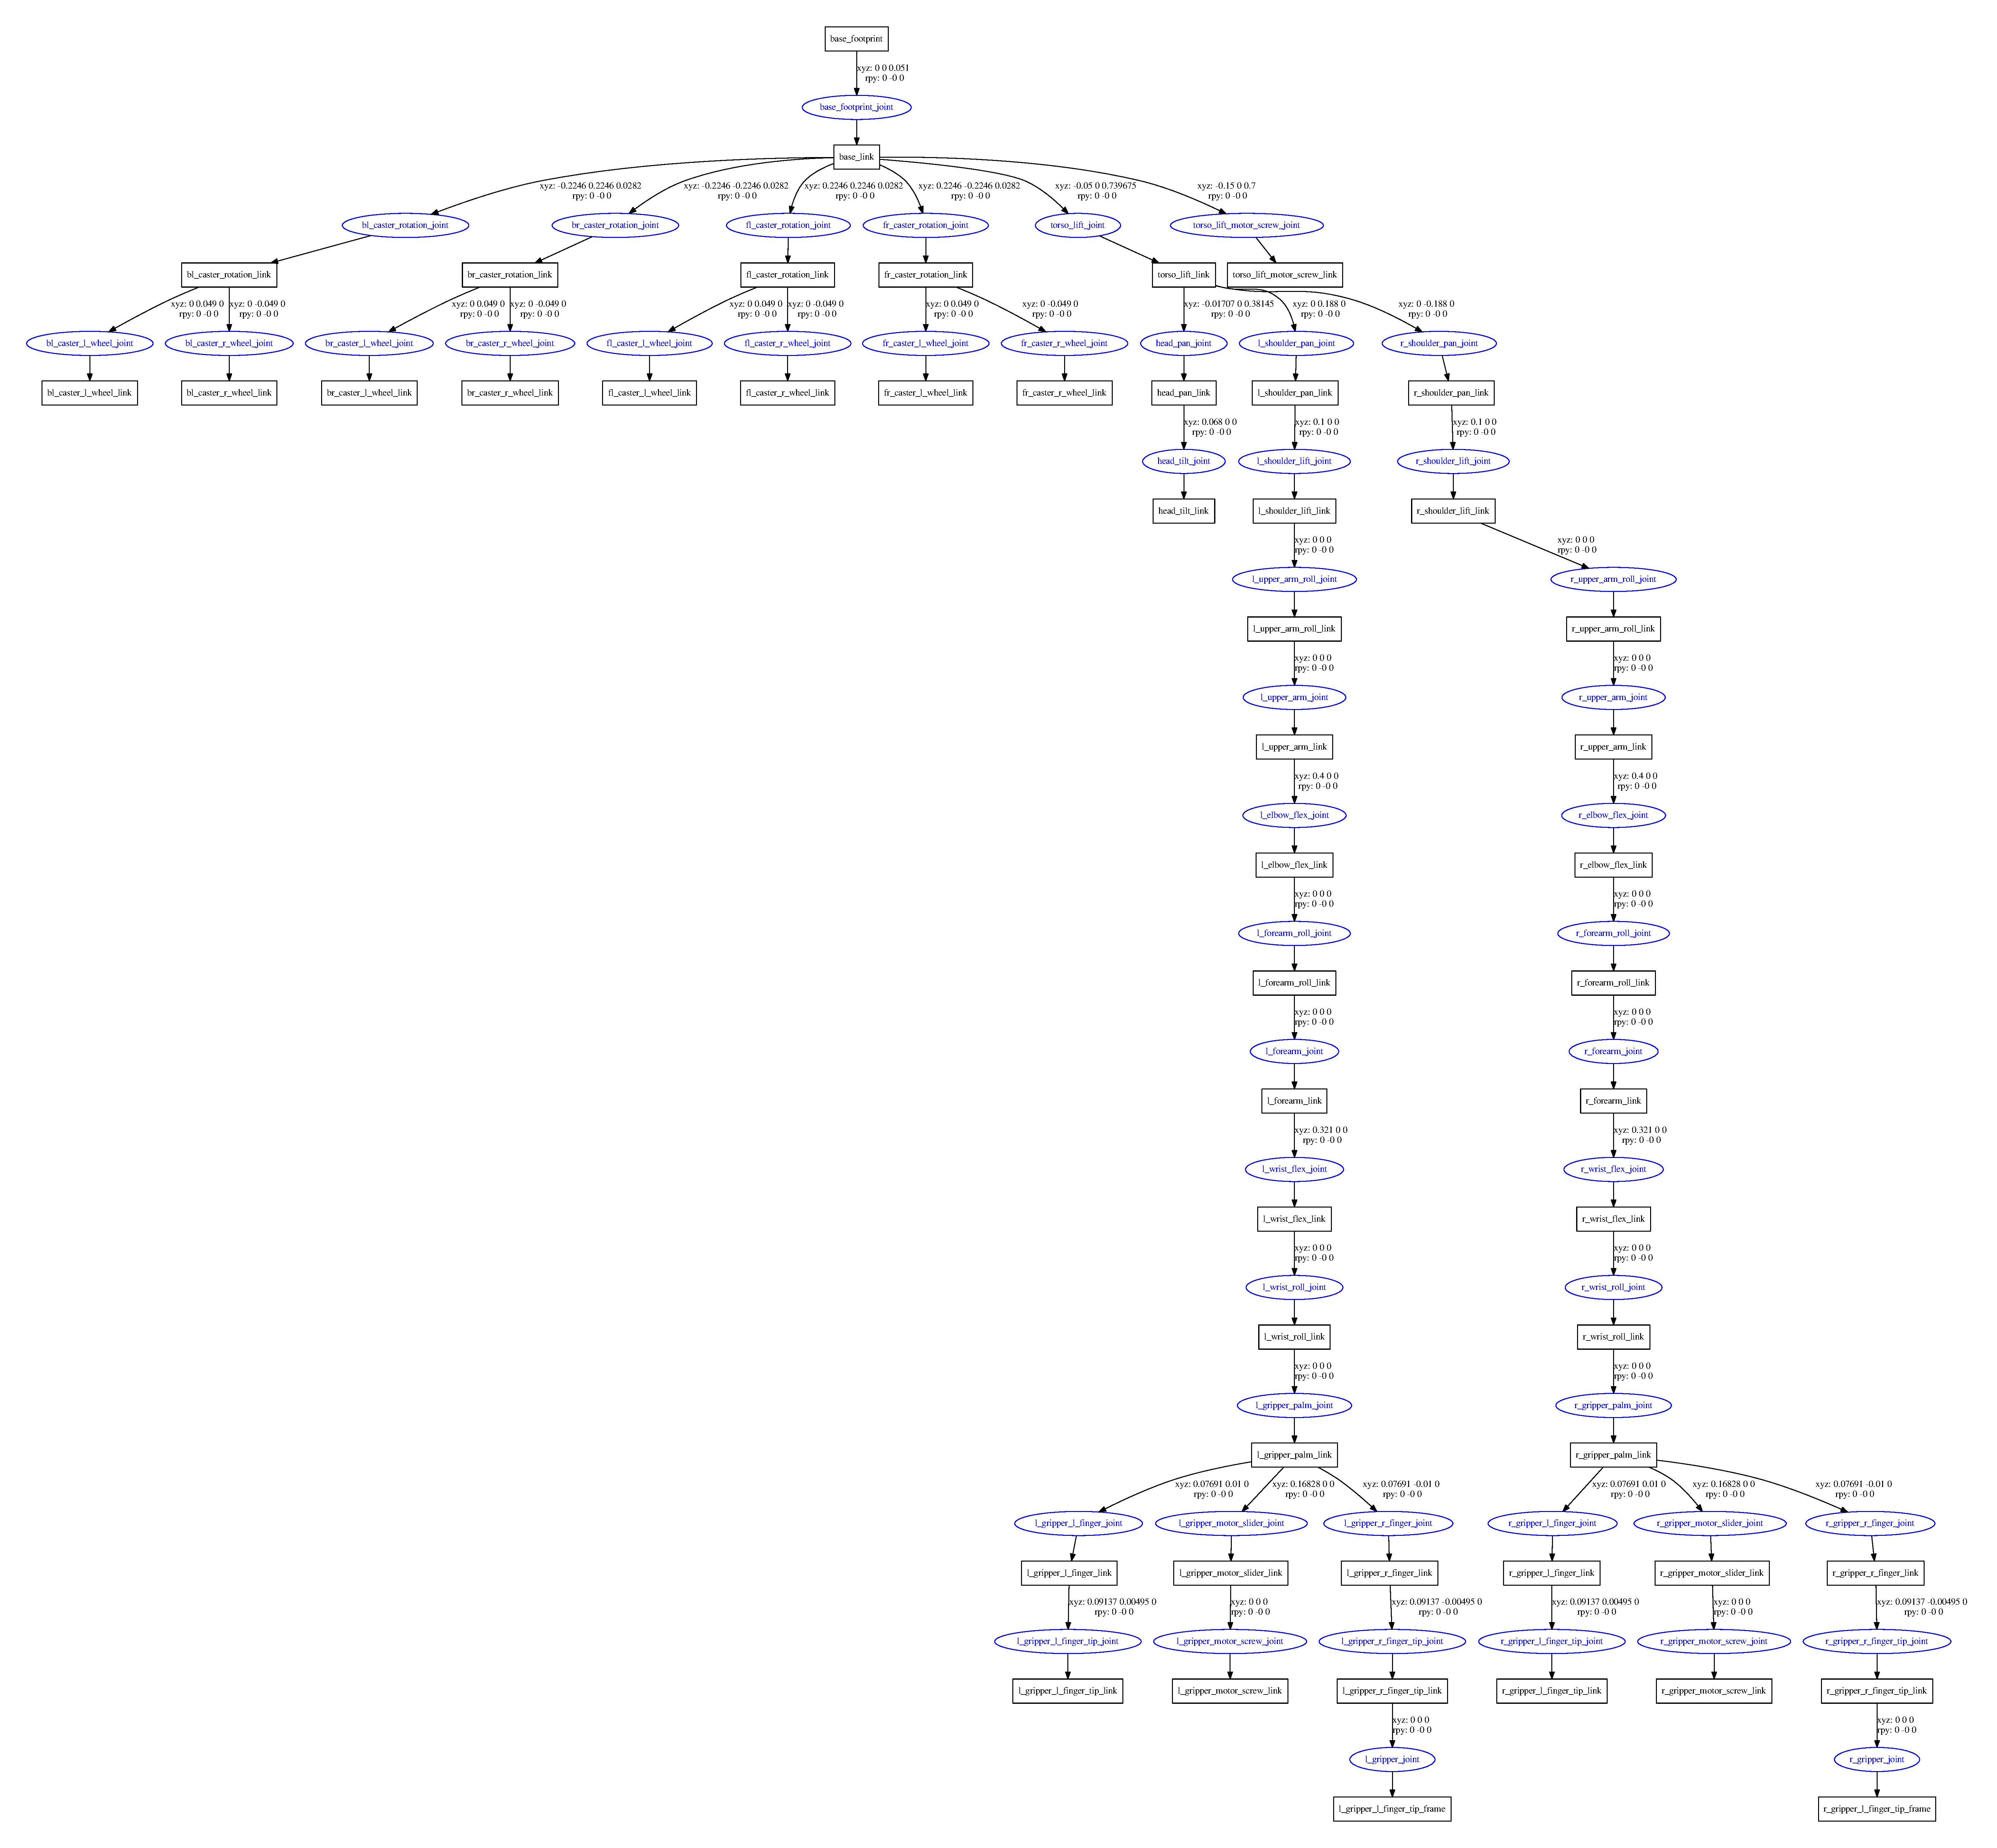
\includepdf[scale=0.95,pages=1,pagecommand=\section{Minimal structure tree}\label{annex:minStruct}]{images/bobbyTree.pdf}


\section{Position data of SIGVerse for an ik movement}\label{annex:dataPos}
\noindent\begin{minipage}{\linewidth}% to keep image and caption on one page
\begin{center}
\begin{tabular}{| l | m{8cm} | c | c |}
\hline
	Position asked & Result SIGVerse & Point name\\\hline
	0 0 -0.1 & 116.64 82.82 41.99 & B \\
	0 -0.1 0 & 116.64 93.83 43.51 & C\\
	0 0 0.05 & 116.64 99.20 41.39 & A\\
	0 0.15 0 & 116.64 93.98 44.83 & D\\
	0 -0.1 -0.1 & 116.64 82.93 43.59 & E\\
	0 -0.1 -0.15 & 116.64 77.59 43.16 & F\\
	0 -0.15 -0.1 & 116.64 83.18 45.33 & G\\
	0 0.1 0.03	& 116.64 97.05 43.05 & H\\
	0 0.16 0 & 116.64 94.24 44.91 & J\\
	0 -0.17 -0.1 & 116.64 83.56 46.09 & K\\
	0 0 -0.08 & 116.64 85.05 42.13 & L\\
	0 0 -0.05 & 116.64 88.38 42.22 & M\\\hline
\end{tabular}
\end{center}
\captionof{table}{Jobs}\label{tab:lots}%      only if needed  
\end{minipage}

\end{document}
